	% !TeX encoding = utf8
	% !TeX program = xelatex
	
	\documentclass[11pt,draft]{article}
	\usepackage[utf8]{inputenc}
	\usepackage[T1]{fontenc}
	\usepackage[english,russian]{babel}
	
	% Insert pdf pages
	\usepackage[final]{pdfpages}
	
	\usepackage{toolbox}
	\usepackage{guitar}
	
	% For  \gchords
	\usepackage{gchords}
	\usepackage{guitarchordschemes}
	
	% For tabs
	\usepackage{musixtex}
	
	% custom clef
	\newcommand\TAB[1]{%
		\setclefsymbol{#1}{\,\rotatebox{90}{TAB}}%
		\setclef{#1}9}
	
	% internal string choosing command
	%  #1: string (a number from 1--6)
	%  #2: finger
	\makeatletter
	\newcommand\@str[2]{%
		\ifcase#1\relax\@strerror
		\or\def\@strnr{-1}%
		\or\def\@strnr{1}%
		\or\def\@strnr{3}%
		\or\def\@strnr{5}%
		\or\def\@strnr{7}%
		\or\def\@strnr{9}%
		\else\@strerror
		\fi
		\zchar\@strnr{\footnotesize#2}}
	% \@strerror could be defined to issue some warning/error
	
	% Disable hyphenation
	\usepackage[none]{hyphenat}
	
	% User level commands
	\newcommand\STr[2]{\@str{#1}{#2}\sk}  % with a full note skip
	\newcommand\Str[2]{\@str{#1}{#2}\hsk} % with a half note skip
	\newcommand\str[2]{\@str{#1}{#2}}     % with no skip
	
	
	%%% Работа с русским языком
	\usepackage[no-math]{fontspec}      %% подготавливает загрузку шрифтов Open Type, True Type и др.
	\defaultfontfeatures{Ligatures={TeX},Renderer=Basic}  %% свойства шрифтов по умолчанию
	\setmainfont[Ligatures={TeX,Historic}]{Times New Roman} %% задаёт основной шрифт документа
	\setsansfont{Helvetica Neue}                    %% задаёт шрифт без засечек
	
	\newfontfamily{\allods}{AllodsWest}
	
	% Set table of contents font
	\usepackage{tocloft}
%	\renewcommand{\cftsecfont}{\normalfont\allods} 
	
	% start each section on its own page
	\usepackage{titlesec}
	\newcommand{\sectionbreak}{\clearpage}
	% Set section title font
	\titleformat{\section}{}{\thesection}{0pt}{\hphantom}
	\titlespacing*{\section}{0pt}{0pt}{-5pt}
	\renewcommand{\cfttoctitlefont}{\Large\allods}
	
	% hide section numbers
	\renewcommand{\thesection}{}
%	\renewcommand{\thesubsection}{\arabic{section}.\arabic{subsection}}
	\makeatletter
	\def\@seccntformat#1{\csname #1ignore\expandafter\endcsname\csname the#1\endcsname\quad}
	\let\sectionignore\@gobbletwo
	\let\latex@numberline\numberline
	\def\numberline#1{\if\relax#1\relax\else\latex@numberline{#1}\fi}
	\makeatother
	
	% Set A5 format
	\usepackage[left=0.5cm,top=0.5cm,right=0.5cm,bottom=2cm,nohead,footskip=0.5cm]{geometry}
	\geometry{a5paper}
	
	% Two columns
	\usepackage{multicol}
	
	\usepackage[parfill]{parskip}    % Activate to begin paragraphs with an empty line rather than an indent
	
	% Header tuning
	\usepackage{fancyhdr}
	\setlength{\headheight}{20pt}
	\renewcommand{\sectionmark}[1]{\markright{#1}}
	\fancyhead[L]{\large\allods\rightmark}
	\renewcommand{\headrulewidth}{2pt}

	\newcommand\invisiblesection[1]{%
		\refstepcounter{section}%
		\addcontentsline{toc}{section}{\protect\numberline{\thesection}#1}%
		\sectionmark{#1}}
	
	\title{Сборник песен обо всём}
	\author{Алексей Найден}
	\date{}
	
	\newcommand{\gcomment}[1]{\textbf{#1}}
	\newcommand{\gauthor}[1]{\fancyhead[R]{\textit{#1} }}
	\newcommand{\gchords}[1]{{\footnotesize #1}}
	\newcommand{\gchorus}[1]{%
		\begin{tcbsiderules}#1\end{tcbsiderules}%
	}
%	\newenvironment{gchorus}
%	{
%			}
%			{
%	
%	}

\usepackage[most]{tcolorbox}
\newtcolorbox{tcbsiderules}[1][]{blanker, breakable, 
	left=3mm,
	borderline west={1pt}{0pt}{black},
	parbox=false,
	#1}

	% Make guitar chords bold
	\renewcommand\guitarPreAccord{\footnotesize\strut\bfseries}
		
	\begin{document}
		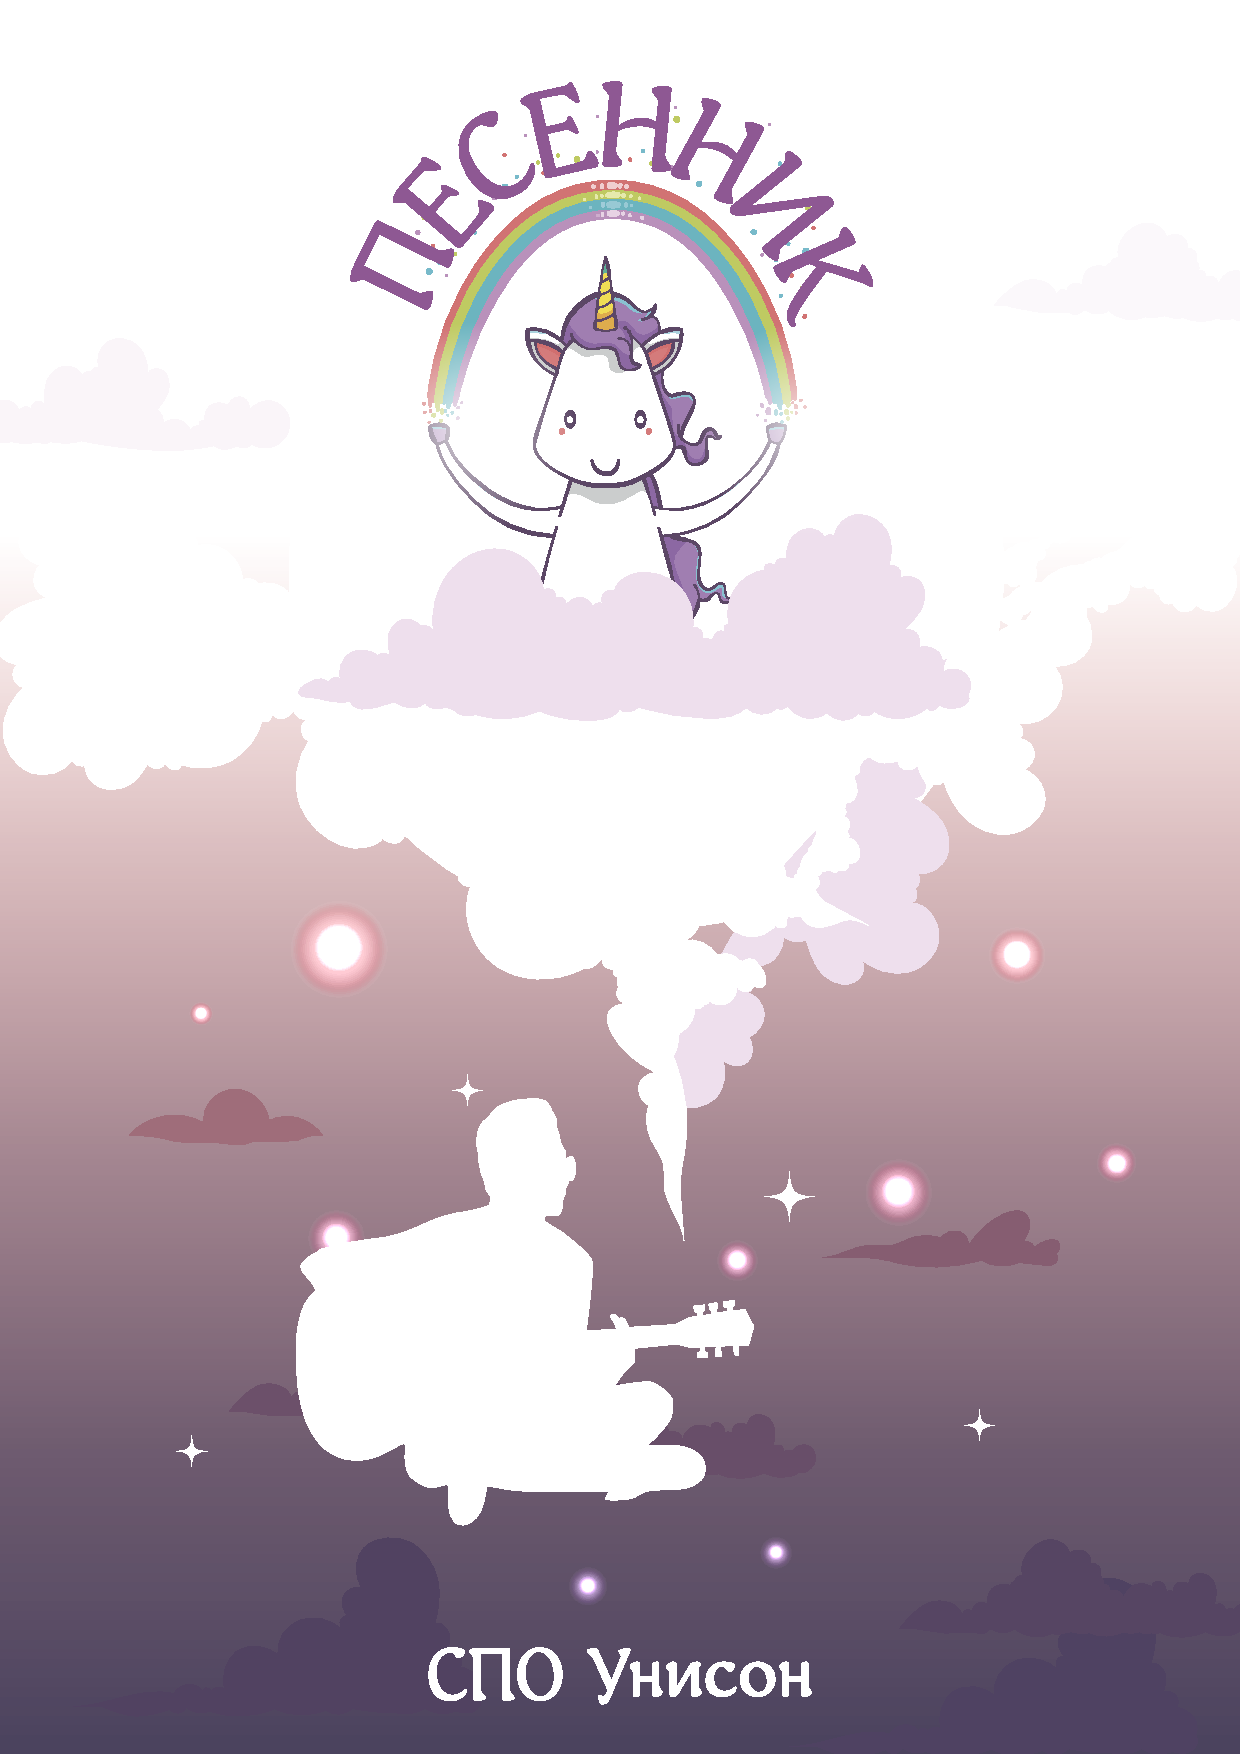
\includepdf[pages={1}]{title.pdf}
%	\begin{titlepage}
%		\vspace*{\stretch{1.0}}
%		\begin{center}
%			\Huge\textbf{Сборник песен обо всём}\\
%			\vspace*{\stretch{2.0}}
%			СПО <<Унисон>>
%		\end{center}
%	\end{titlepage}

	\newpage
	\pagestyle{empty}
	\begin{center}
	  {\Huge \textbf{Благодарности}}
	  
	  \vspace{1em}
	  {\huge
	  За неоценимую помощь в создании этого чудесного кладезя песен, всестороннюю поддержку и бесконечную любовь к гитаре огромная благодарность и теплейшие фиолетовые объятия передаются Яновой Алене Витальевне, Лебедеву Олегу Викторовичу, Лежниной Юлии Геннадьевне, Астафьевой Анне Юрьевне, Исиченко Олесе Константиновне, Найдену Алексею Владимировичу и Николаевой Дарье Михайловне.
	
	  \vspace{1em}
	  Используйте песенник мудро: пойте душевно, играйте громко, дарите волшебную атмосферу и уют всем вокруг!
	
	  \vfill
	  Автор \textit{Шпарута Софья Константиновна}
	}
	\end{center}
	\newpage
		\pagestyle{plain}
	
	\tableofcontents

	\section{3 полоски}
	\pagestyle{fancy}
	\renewcommand{\sectionmark}[1]{\markright{#1}}
	
	\gauthor{Animal Jazz}
	  \begin{guitar}
	    \gcomment{Вступление}: \gchords{ Dm Dm B F (2р)} 
	
	    [Dm]Как же произошло –
	    [B]Жизнь опять, словно [F]белый лист,
	    [Dm]Мажет красками холст
	    [B]Красно-желтым – е[F]е каприз?
	
	    [Dm]Ночь все перевернет
	    [B]И оставит боль [F]на потом.
	    [Dm]Точно еще повезет 
	    C [B]те[F]плом. [С]{ }
	
	      \gcomment{Припев:}%
	      \gchorus{
	      [F]Джинсы порезаны, [Dm]лето,
	      Три полоски на [Am]кедах
	      Под теплым дож[B]дем\dots
	      Ты снова лучше всех,
	      А дачу, маму, билеты
	      Мы переживем\dots}
	
	     \gcomment{Проигрыш:} \gchords{Dm Dm B F С} (2р)
	
	    Зайди в знакомый подъезд,
	    Поднимись на восьмой этаж.
	    Смотри, как солнышко ест
	    Этот мир – он уже не наш.
	    Скоро наступит сентябрь,
	    SMS'ом пришлет пароль.
	    Он оденет тебя в новую любовь
	
	      \gcomment{Припев} (2р)
	      
	    [Am]Лишь [B]несколько слов [F]могут [Dm_]у[C]бить,
	    Но, если веришь в любовь, стоит еще жить.
	    Лишь несколько слов могут убить,
	    Но, если веришь в любовь, стоит еще\dots
	
	      \gcomment{Припев} (2р)
	      \gcomment{Кода:} \gchords{Bm}
	  \end{guitar}
	\section{10 капель}
	\gauthor{Танцы минус}
	
	\begin{guitar}
	  \gcomment{Вступление}:  \gchords{C E Am F}
	
	  [C]Десять капель дож[E]дя y тебя на пле[Am]че,
	  Ты забыла свой [F]зонт, ты спешила ко [C]мне.
	  Десять капель дож[E]дя на плече y теб[Am]я,
	  Десять капель люб[F]ви, десять капель ог[C]ня.
	
	  \gcomment{Проигрыш}: \gchords{C E Am F} (2р)
	
	  Время делает шаг, время делает круг,
	  Мы забудем друзей, мы забудем подруг.
	  Просто выпьем вина из любви и огня.
	  Десять капель меня, десять капель тебя.
	
	  \gcomment{Припев}:%
	  \gchorus{
	  [C]Твоя[E] ладонь[Am] горит[F] в моих руках,
	  Любви пожар в твоих глазах.%
	}%
	  
	  \gcomment{Проигрыш}
	
	  Голос твой в тишине околдует меня,
	  Ярким жарким огнем стану я до утра.
	  Ты прикажешь: “Гори” – и я вспыхну любя.
	  B этом пламени ты, в этом пламени я.
	
	  \gcomment{Припев}
	  \gcomment{Проигрыш}
	\end{guitar}
	
	\section{Батарейка}
	\gauthor{Жуки}
	
	\begin{guitar}
	  \gcomment{Вступление}: \gchords{Hm A G F$\sharp$} (2р)
	
	  [Hm] Холодный [A]ветер с дож[G]дем усилил[F\#]ся стократно,
	  Все говорит об одном, что нет пути обратно,
	  Что ты не мой лопушок, а я не твой Андрейка,
	  Что у любви у нашей села батарейка.
	
	 \gcomment{Припев:}%
	 \gchorus{
	  [Hm] О-[A]оу-и-я-и-[G]е! [F\#]Батарейка
	  О-оу-и-я-и-е! Батарейка%
		}%

	  Я тосковал по тебе в минуты расставания,
	  Ты возвращалась ко мне сквозь сны и расстояния,
	  Но, несмотря ни на что, пришла судьба-злодейка,
	  И у любви у нашей села батарейка.
	
	  \gcomment{Припев}
	  \gcomment{Проигрыш}: Hm A G F$\sharp$ (2р)
	
	  И вроде все как всегда: все те же чашки-ложки,
	  Все та же в кране вода,
	  Все тот же стул без ножки,
	  И все о том же с утра щебечет канарейка,
	  Лишь у любви у нашей села батарейка.
	
	  \gcomment{Припев} (2р)
	
	\end{guitar}
	
	\section{Белая гвардия}
	\gauthor{Зоя Ященко}
	
	\begin{guitar}
	\gcomment{Вступление}: Am D7 G C Am H7 Em (2р)
	
	[Em]Белая гвардия, белый снег,
	[Am7]Белая музыка революции,
	[D7]Белая женщина, нервный смех,
	[G]Белого платья слегка коснуться.
	
	Белой рукой распахнуть окно,
	Белого света в нем не видя,
	Белое выпить не до дна вино,
	В красную улицу в белом выйти.
	
	\gcomment{Припев:}%
	\gchorus{
	Ког[Em]да ты вернешься – все будет и[Am]наче,
	И нам не узнать друг друга,
	Ког[D7]да ты вернешься, а я не же[G]на
	И даже не подруга.
	Ког[C]да ты вернешься ко мне, так бе[Am]зумно
	Тебя любившей в прошлом,
	Ког[H7]да ты вернешься – увидишь, что [Em]жребий
	Давно и не [Е7]нами брошен.%
}%
	
	\gcomment{Проигрыш:} \gchords{Am  D7  G  C  Am  H7  Em} (2р)
	
	Сизые сумерки прошлых лет
	Робко крадутся по переулкам.
	В этом окне еле брезжит свет.
	Ноты истерзанны, звуки гулки.
	
	Тонкие пальцы срывают аккорд\dots
	Нам не простят безрассудного дара.
	Бьются в решетку стальных ворот
	Пять океанов земного шара.
	
	\gcomment{Припев}
	
	Красный трамвай простучал в ночи.
	Красный закат догорел в бокале.
	Красные-красные кумачи
	С красных деревьев на землю пали.
	
	Я не ждала тебя в октябре,
	Виделись сны, я листала сонник.
	Красные лошади на заре
	Бились копытами о подоконник.
	
	\gcomment{Припев:}
	Когда ты вернешься – все будет иначе,
	И нам не узнать друг друга,
	Когда ты вернешься, а я не жена
	И даже не подруга.
	Когда ты вернешься, вернешься в наш город
	Обетованный.
	Когда ты вернешься, такой невозможный
	И такой желанный.
	
	\gcomment{Проигрыш}
	\end{guitar}
	
	\section{Боже, какой пустяк}
	\gauthor{Александр Иванов}
	
	\begin{guitar}
	  \gcomment{Вступление}:
	  \gchords{Am | Am/G | D}
	  \gchords{D | Dm | Dm/H | E | E}
	
	[Am]Я вижу небо, в [Am/G]нем тишина,
	Я подни[F]маюсь к небу, [Dm]еле ды[E]ша.
	И вд[Dm7]руг понимаю -- [G]это во [C]мне ду[Am]ша.
	[Dm7]Странное дело -- [G]это моя ду[C]ша. [E7]{ }
	
	Как нелепо, жить вниз головой,
	Когда такое небо есть надо мной,
	И, кажется, звезды можно достать рукой.
	Я и не ведал, что этот мир такой.
	
	\gcomment{Припев:}%
	\gchorus{
	Боже, ка[Am]кой пус[Am/G]тяк,
	Сделать хоть [D/F\#]раз что-нибудь не [D]так:
	Выкинуть [Dm]хлам из дома
	И [G]старых позвать дру[C]зей. [E7]{ }
	
	Но что-то всерьез менять,
	Не побоясь в мелочах потерять,
	Свободно только небо
	[Dm/H]Над головой мо[E7]ей.%
}%
	
	Я был богом в прошлую ночь,
	Я отыскал дорогу и выбежал прочь –
	Богом стать просто, если уже невмочь,
	И не над чем плакать, дом покидаю в ночь.
	
	Но оказалось даже тогда,
	Что все дороги света ведут в никуда.
	И даже, когда под ногами блестит вода,
	Бог просто не может странником быть всегда.
	
	\gcomment{Припев}
	\gcomment{Проигрыш:}
	\gchords{Am Am/G F Dm E}
	\gchords{Dm7 G C Em7 Am}
	\gchords{Dm7 G C Hm7 E}
	
	[Hm]Я поднимаю [Hm/A]свой воротник,
	Ругаю [G]дождь и слякоть, [Em]будто ста[F\#]рик,
	Бе[Em7]гу за толпою, [A]видно уже при[D]вык. [Hm]{ }
	И в [Em7]памяти небо, [A]как нереальный [D]блик. [F#7]{ }
	
	Но однажды мне станет легко,
	И будет все неважно и далеко,
	Меня примет небо в свой неземной покой,
	И я стану просто облаком над рекой.
	
	\gcomment{Припев:} (2р)%
	\gchorus{
	Боже, ка[Hm]кой пус[Hm/A]тяк,
	Сделать хоть [E/G\#]раз что-нибудь не [E]так:
	Выкинуть [Em]хлам из дома
	И [A]старых позвать [D]друзей. [F\#7]{ }
	
	Но что-то всерьез менять,
	Не побоясь в мелочах потерять,
	Свободно только небо
	[Em/C\#]Над головой мо[F\#7]ей.%
	}
	
	\gcomment{Кода:} \gchords{Hm}
	\end{guitar}
	
	      
	\section{В парусиновых брюках}
	\gauthor{Альфред Тальковский}
	
	\begin{guitar}
%	%\begin{multicols}{2}
	В пару[Am]синовых брюках, 
	Широких, залатанных, длинных                                        
	Мы хо[A7]дили вразвалку –                      
	Чуть набок была голо[Dm]ва,                  
	Мы придумали [G7]море –                        
	Та[C]ким, как на старых кар[Am]тинах,                               
	И ус[Dm]ловились так,                             
	Что отк[E7]рыты не все остро[Am]ва, остров[А7]а.                          
	Мы придумали [G7]море –                        
	Та[C]ким, как на старых кар[Am]тинах,                               
	И ус[Dm]ловились так,                             
	Что отк[E7]рыты не все остро[Am]ва.   
	
	Мы придумали город, 
	Где сушатся старые сети, 
	Где вокзал и причал 
	Одинаково рыбой пропах.
	Мы придумали город, 
	В котором суровые дети, 
	И развешаны компасы 
	Вместо часов на столбах. 
	
	Мы придумали честность – 
	Такую, что дай Бог любому. 
	Если с кем-то беда, 
	Ты попробуй-ка спрятать глаза.
	Если крик за окном, 
	Ты попробуй не выйти из дома, 
	Если в шторм тонет кто-то, 
	Попробуй гасить паруса. 
	
	А потом – так положено, 
	Возраст такой наступает: 
	Вырастаем из улочек детства, 
	Из доброй мечты. 
	Стрелка полюс меняет, 
	И город придуманный тает, 
	И пора уходить, 
	И пора нам сжигать корабли.
	
	Только я обманул, 
	Я причёску сменил и походку, 
	Ну а парусник сжёг… 
	Чтоб пахуча была и крепка, 
	Золотою янтарной 
	Смолой просмолил свою лодку, 
	И отправил на ней 
	По морям своего двойника. 
	
	Эта лодка приходит
	Не в солнечный день, а в ненастье… 
	Только знаю: 
	Если глаза мне застелет туман, 
	Если я промолчу,
	Отвернусь от чужого несчастья, 
	Город мой, моё имя 
	И лодку сожжет капитан.
%	%\end{multicols}
	\end{guitar}
	
	\section{Вахтерам}
	\gauthor{Бумбокс}
	
	\begin{guitar}
	  \gcomment{Вступление}: \gchords{Am G Dm E7}
	
	Тебе не нравится [Am]дым, и черт с ним.            
	Он убивает сло[G]ва, кругом голова.              
	Уже разносит мол[Dm]ва по дворам,               
	Что между нами чи[E7]вава.
	
	О чем с тобой говорить, потеряли нить.
	Быть не собой перестать и дома спать.
	Нас не измерить на глаз, а сейчас
	Зачем мы давим на тормоз, не на газ?
	
	Вопрос извечный: зачем да почему?
	Я понемногу с ума, ты не сама.
	А эти ночи в Крыму – теперь кому?
	Я, если встречу, потом передам ему.
	
	Писклявый твой голосок, как электрошок.
	Что я бухой без вина - твоя вина.
	Теперь узнает страна до темна - 
	Им донесут обо всем на FM-волнах.
	
	\gcomment{Припев:}%
	\gchorus{
	Я помню [Am]белые обои, [C]черная посуда,                 
	[Dm]Нас в хрущевке двое,[E7] кто мы и откуда, откуда?              
	[Am]Задвигаем шторы, [C]кофеек, плюшки стынут.                  
	[Dm]Объясните теперь нам, вахтеры,
	[E7]Почему я на ней так сдвинут?%
}%
	
	Давай вот так просидим до утра.
	Не уходи, погоди, но мне пора.
	И если выход один впереди,
	То почему мы, то холод, то жара?
	
	Раскладывать по местам я устал
	И поворачивать вспять – ну вот опять –
	Прикосновения плавили мой метал.
	Ты элемент номер пять - ни дать, ни взять.
	
	Идет к финалу игра в этот раз,
	А ты все так же молчишь, я говорю.
	Минут пятнадцать осталось до утра - 
	Не вызывай так словлю и свалю.
	
	Попробуем все подшить, не ворошить,
	Мобильные номера постирать,
	А уходить, не спросив - нету сил.
	Давай попробуем заново все собрать.
	
	\gcomment{Припев:}%
	\gchorus{
	Белые обои, черная посуда,                 
	Нас в хрущевке двое, кто мы и откуда, откуда?              
	Задвигаем шторы, кофеек, плюшки стынут.                  
	Объясните теперь нам, вахтеры,
	Почему я на ней так сдвинут?%
}%
	
	Я помню белые обои, черная посуда,                 
	Нас в хрущевке двое, кто мы и откуда, откуда?              
	Задвигаем шторы, кофеек, плюшки стынут.                  
	Объясните теперь нам, вахтеры,
	Почему я на ней так сдвинут?
	
	Белые обои, черная посуда,                 
	Нас в хрущевке двое, кто мы и откуда, откуда?              
	Задвигаем шторы, кофеек, плюшки стынут.                  
	Объясните теперь нам, вахтеры,
	Почему я на ней так сдвинут?
	\end{guitar}
	
	\section{Вера в чудо}
	\gauthor{Алексей Носов}
	
	\begin{guitar}
	\gcomment{Вступление}: \gchords{Hm F$\sharp$m G D A} (2р)
%\begin{multicols}{2}
	
	[Hm]Дождь, темно и уныло.
[F\#m]Ждешь, устала, простыла.                         
[G]Я останусь сегодня о[D]дин,                    
Но [A]ты все равно прихо[Hm]ди.                    
Ведь это не важно. [F\#m]Да,                 
Пусть разные горо[G]да
И долгие поез[D]да.
Но [A]даже не нужно [Hm]ждать,
А просто поверить, [F\#m]знать -  
Не заперты двери.                     
[G]И прозрачною каплей [D]вниз,
[A]Перьями птиц.

\gcomment{Припев:}%
\gchorus{
[Hm]Береги веру в [F\#m]чудо, буду,                  
[G]Наверно, не [D]раз еще [A]буду                            
[Hm]Выглядеть очень ус[F\#m]талым, осталось [G]мало,                     
Весь по горо[D]дам по вок[A]залам.       
[Hm]Долгие до[F\#m]роги к небу                       
[G]И мы все время бе[D]жим,а [A]мне бы             
Ды[Hm]шать, просто ды[F\#m]шать тобою,             
В[G]се до[D]верив ге[A]роям.%
}


Дни, плетем паутину.
Вне рисуют картины сны.
Дороги, усталость, боль,
Предчувствие встречи, любовь.
Душа не остынет пусть,
Волною нахлынет грусть,
Останусь сегодня один,
А ты все равно..

\gcomment{Припев}

\gcomment{Кода:} 
\gchords{Hm F$\sharp$m G D A} (2р)
\gchords{Hm}

%\end{multicols}

	
	\end{guitar}
	
	\section{Верхом на звезде}
	\gauthor{Найк Борзов}
	
	\begin{guitar}
	Верхом на [G]звезде, 	        
	Вцепившись в [Hm]лучи,                        
	С лу[Am]ной на повод[C]ке, в но[Hm]чи, [D]{ }
	
	Верхом на звезде	           
	Несусь навстречу ветрам           
	К несбывшейся мечте и сна-[C]а-[D]ам 
	
	\gcomment{Припев:}%
	\gchorus{
	[Em] О, жизнь, ты пре[C]красна!                           
	[G] О, жизнь, ты пре[D]красна впол[Em]не,                        
	Бываешь не[Am]много о[C]пасна, оу-[D]е.
	                 
	Возьми мое сердце,
	Храни, вспоминай обо мне.
	Поверь мне, что все не напрасно.%
}%
	         
	Верхом на звезде,
	Над лесом рекой
	Потерян навсегда покой. 
	Верхом на звезде,
	Mi torno diablo esta,
	Билет в один конец, весна
	
	\gcomment{Припев}
	\gcomment{Проигрыш:} \gchords{G Hm C Cm Cm7 D D7}
	        
	Верхом на звезде
	Несусь навстречу ветрам,
	И создал этот мир я [G]сам [Hm|]{ } [D]{ }
	
	\gcomment{Припев}
	Верь [Gm]мне
	\end{guitar}
	
	\section{Ветер}
	\gauthor{ДДТ}
	
	\begin{guitar}
	\gcomment{Вступление}: \gchords{Em C Am D} (4р)
	                           
	[Em] О, прекрасная [D]даль, поглотившая [Em]небо. [C|]{ } [Am|]{ } [D]{ }
	Облака, как к любимой, прижались к земле,
	[Em] Где ты и я под прос[C]той да не[D]скошенной [Em]крышей [C|]{ }[D]{ }
	[Em]Ищем[C] друг в [D]друге теп[Em]ло. [C] Что, [Am]что\dots
	
	\gcomment{Припев:}%
	\gchorus{
	[D]Что нам [G]ветер[D]  да на это отв[Em_]ет[C]ит,
	Несущийся [G]мимо[D]  да сломавший кры[G]ло? [C]{ } 
	И, у[D]пав между [G]нами,[D] так недолго лю[Em]бимых,[C]{ }
	Разбил он объ[G]ятья,[D] как простое сте[Em]кло.%
}%
	
	\gcomment{Проигрыш:} \gchords{Em C Am D/F$\sharp$} (4р) 
	
	Мы стояли на прошлом, мы ждали начала,
	Прижимаясь к стене, где исчезли они,
	Где еще одну жизнь одна смерть обвенчала
	Парой вспышек огня, да в эти смутные дни.
	
	\gcomment{Припев}
	\gcomment{Проигрыш} (2р)
	\gcomment{Припев}
	\gcomment{Проигрыш}
	\gcomment{Кода:} \gchords{Em}
	\end{guitar}
	
	\section{Вечер бродит}
	\gauthor{Ада Якушева}
	
	\begin{guitar}
	[Am]Вечер [Dm]бродит [E]по лесным [Am]дорожкам.                   
	[Am]Ты ведь [Dm]тоже [G]любишь вече[C]ра.                   
	[A7]Подожди, пос[Dm]той ещ[G]е не[C]множко,                     
	[Dm]Посидим с товарищами [Am|]у [E]кос[Am]тра. 
	[A7]Подожди, пос[Dm]той ещ[G]е не[C]множко,                     
	[Dm]Посидим с товарищами [Am|]у [E]кос[Am]тра.
	
	Вижу целый мир в глазах тревожных 
	В этот час на берегу крутом. 
	Hе смотри ты так неосторожно – 
	Я могу подумать что-нибудь не то.
	
	Вслед за песней позовут ребята 
	В неизвестные еще края, 
	И тогда над крыльями заката 
	Вспыхнет яркой звездочкой мечта моя. 
	
	Ясный месяц на прогулку вышел, 
	Светят звезды из глубин небес. 
	Друг хороший рыжий, ты меня услышишь – 
	Эту песню я сейчас пою тебе. 
	
	Знаю, будут и другие встречи, 
	Год за годом пролетят года, 
	Hо вот этот тихий теплый вечер 
	Мы с тобою не забудем никогда.
	\end{guitar}
	
	\section{Владивосток 2000}
	\gauthor{Мумий Тролль}
	
	\begin{guitar}
	\gcomment{Вступление}: \gchords{Am}
	
	С гра[Am]натою в кармане, с чекою в руке,
	Мне чайки здесь запели на знакомом языке. 
	Я [Dm]отходил спокойно, не прятался, не вор.                       
	Ко[C]лесами печально в небо [E]смотрит круизер.
	
	Когда туман растаял и проныла луна,
	Со смены не вернулась молодая жена.
	Вода отравится, погаснет свет, утихнет звук.
	К тебе я больше не вернусь - 
	Такой теперь я друг.
	
	\gcomment{Припев:}%
	\gchorus{
	     У[Am]ходим, уходим, у[Dm]ходим,                  
	     На[C]ступят времена по[E]чище.                
	     Бь[Am]ется родная, в экс[Dm]тазе пылая, [C]{ }
	     Владивосток две [E]тыщи.}
	
	В объятьях полупьяных женщин гибли моряки,
	Тельняшки рвали и кололи прямо на груди.
	Мне сердце остановится, не будет слышен стук.
	Ты свой последний танец танцевал уже без рук.
	
	Быть может, откопают через тысячу лет
	В фантиках жвачки и осколках монет,
	Где вылизан весь берег, не дошел до волны,
	Где рельсы вылезали из кармана страны.
	
	\gcomment{Припев} (2р)
	\gcomment{Кода:} 
	     У[Am]ходим, уходим, у[Dm]ходим\dots [C|]{ }[E]{ } (2р)
	     [Am]{ }
	\end{guitar}
	
	\section{Восьмиклассница}
	\gauthor{Кино}
	
	\begin{guitar}
	\gcomment{Вступление}: \gchords{Am Em} (4р) 
	            
	Пус[Am]тынной ули[Em]цей вдвоем                
	С тоб[C]ой куда-то [G]мы идем,                 
	[F]Я курю, а [G]ты кон[C]феты ешь.
	            
	И светят фонари давно,
	Ты говоришь: <<Пойдем в кино>>,
	А я тебя зову в кабак, конечно.
	
	\gcomment{Припев:}%
	\gchorus{
	[F]М-ммм[G]м, восьми[C]классница а-a-[Am]а,          
	[F]М-ммм[G]м\dots}
	
	\gcomment{Проигрыш:} \gchords{Am  Em} (4р) 
	
	Ты говоришь, что у тебя
	По географии трояк,
	А мне на это просто наплевать.
	Ты говоришь, из-за тебя
	Там кто-то получил синяк --
	Многозначительно молчу, и дальше мы идем гулять.
	
	\gcomment{Припев}
	\gcomment{Проигрыш} 
	
	Мамина помада,
	Сапоги старшей сестры,
	Мне легко с тобой, а ты гордишься мной.
	Ты любишь своих кукол
	И воздушные шары,
	Но в десять ровно мама ждет тебя домой.
	
	\gcomment{Припев}
	\gcomment{Проигрыш} 
	\end{guitar}
	
	\section{Вот пуля просвистела}
	\gauthor{Чиж \& Co}
	
	\begin{guitar}
	\gcomment{Вступление}: \gchords{Am Am Am G} (4р)
	                                 
	Вот [Am]пуля просвистела, в грудь по[C]пала мне,                           
	[Dm]Спасся я в степи я на ли[Am]хом ко[G]не,                        
	Но шашкою меня комиссар достал,
	Покачнулся я и с коня упал.
	
	\gcomment{Припев:}%
	\gchorus{                    
		[Am]Хэй, [G]ой да, [C]конь мой воро[A7]ной.                  
		[Dm]Хэй, да об[Am]рез сталь[G]ной.                  
		[Am]Хэй, да [G]ты, гус[C]той ту[A7]ман.                   
		[Dm]Хэй, ой да, [F]батька-[G]ата[Am]ман.            
		Да [F]батька-[G]ата[Am]ман.}
	
	На одной ноге я пришел с войны,
	Привязал коня, сел я у жены.
	Но часу не прошло - комиссар пришел,
	Отвязал коня и жену увел.
	
	\gcomment{Припев}
	\gcomment{Проигрыш:}
	 \gchords{Am Am Am G} (2р)
	 \gchords{Am C Dm Am G} (2р)
	\gcomment{Припев}
	
	Спаса со стены под рубаху снял,
	Хату подпалил, да обрез достал.
	При Советах жить - торговать свой крест.
	Сколько нас таких уходило в лес.
	
	\gcomment{Припев}
	\gcomment{Кода:} 
	 \gchords{Am Am Am G} (2р)
	 \gchords{Am}
	\end{guitar}
	
	\section{Все расстояния}
	\gauthor{Михаил Бесчальник}
	
	\begin{guitar}
	[Am]Все расстояния когда-нибудь в круг замы[E]каются.
	[E7]Все из разлук обязательно встречей кон[Am]чаются. [A7]{ }
	Должны про[Dm]плыть вокруг Зем[G]ли,                        
	Вернуться в [C]гавань кора[Am]бли,                               
	Все поез[Dm]да в свои вер[E]нуться горо[Am]да. [A7]{ }
	Должны про[Dm]плыть вокруг Зем[G]ли,                        
	Вернуться в [C]гавань кора[Am]бли,                               
	Все поез[Dm]да в свои вер[E]нуться горо[Am]да.
	
	Шумный вокзал то встречает друзей, то прощается. 
	Мы расстаемся и снова назад возвращаемся, 
	Чтоб снова стать в орлятский круг, 
	Чтоб снова знать, что рядом друг, 
	И песни петь, чтоб больше не было разлук.
	
	Все расстояния когда-нибудь в круг замыкаются. 
	Все из разлук обязательно встречей кончаются. 
	И через год, и через пять 
	Мы с вами встретимся опять, 
	Ничто не сможет нашей встрече помешать.
	\end{guitar}
	
	\section{Выхода нет}
	\gauthor{Сплин}
	
	\begin{guitar}
	\gcomment{Вступление}: \gchords{Em C G} (4р)
	                     
	[C] Сколько лет про[G]шло,                  
	Все о [D]том же гу[Em]дят провода,
	[C] Все того же [G]ждут само[D]леты.                   
	Девочка с глазами 
	Из самого синего льда  
	Тает под огнем пулемета.
	[C] Должен же рас[G]таять хоть [D]кто-то\dots
	
	\gcomment{Припев:}%
	\gchorus{
	        Скоро рас[Em]свет,        
	        Выхода [С]нет,                   
	        Ключ повер[G]ни и поле[D]тели.
	        Нужно вписать
	        В чью-то тетрадь
	        Кровью, как в метрополитене:              
	        <<Выхода [C]нет>>. [D]{ }
	        Выхода [Em]нет!}
	
	Где-то мы расстались, не помню, в каких городах,
	Словно это было в похмелье.
	Через мои песни идут, идут поезда,
	Исчезая в темном тоннеле.
	Лишь бы мы проснулись в одной постели\dots
	
	\gcomment{Припев}
	\gcomment{Проигрыш:} \gchords{Em C G} (4р)
	
	Сколько лет пройдет, 
	Все о том же гудеть проводам,
	Все того же ждать самолетам.
	Девочка с глазами из самого синего льда
	Тает под огнем пулемета.
	Лишь бы мы проснулись с тобой в одной постели…
	
	\gcomment{Припев}
	\gcomment{Кода:}
	[С] Выхода [G]нет,          
	[D] Выхода [Em]нет!
	
	\gchords{Em C G} (4р)
	\end{guitar}
	
	\section{Гимн ССО ЛЭТИ}
	\begin{guitar}
	\gcomment{Вступление}: \gchords{Em A F G H} (2р)
	
	[Em]Все! Окончен по[G]следний эк[A]замен,                  
	[Em]Вновь реет от[G]рядное [A]знамя,               
	[C]Вновь дороги зо[G]вут нас туда,                   
	Где [F]сильные руки нуж[H7]ны. 
	Пусть другие ищут славу, 
	Нам все по плечу и по нраву, 
	Дарит нам золотые лучи 
	Утро родной страны. 
	 
	\gcomment{Припев:}%
	\gchorus{
	[Em]Нам не [Am]знать покоя,         
	[D]Жизнь не[G]много стоит,     
	[C]Если [F]ты не строил,            
	[F\#]А сидел в теп[H]ле. 
	Петь и делать дело,
	Чтоб спина болела,
	Чтобы вновь хотелось, вновь хотелось             
	[F\#]Жить на [H]этой зем[Em]ле.}
	 
	В путь! И все сомненья отбросим, 
	Мы легкой работы не просим. 
	Первый дом, как большая любовь, 
	Вечно помнится нам. 
	Мы втрое сильней, если надо, 
	Нам счастье людское награда, 
	На мозолистых наших руках
	Солнце будущих дней. 
	 
	\gcomment{Припев}
	 
	Пусть нас караулят дипломы, 
	Но нам не сидеть больше дома, 
	Манит нас в неизвестную даль 
	Слово простое - <<отряд>> (Унисон).
	Пусть все это трудно и сложно, 
	Мы всюду придем и поможем, 
	Чтобы помнили люди всегда 
	Нас, мат-мех, Унисон.
	
	\gcomment{Припев}
	\end{guitar}
	
	\section{Грязные корпуса}
	\gauthor{СПО <<Мишка>>}
	
	\begin{guitar}
	В [С]лагере Дружных,  
	Где бу[Am]зят пионеры, 
	Жил [Dm]парень-вожатый -  
	Же[G]лезные нервы. 	
	И часто бывало 
	Ходили обходы, 
	И в шкаф убирал он 
	Пиво и воды.
	
	\gcomment{Припев:} %
	\gchorus{
	[C]Грязные [Am]корпуса (Обход!)         
	[C]Грязные [Am]корпуса (Плюс СЭС!)                   
	[Dm]Грязные [G]корпуса, корпу[C]са 
	(Обход плюс СЭС равно ***ец!)}
	
	А этажом выше, 
	В такой же вожатской 
	Жили девчонки, 
	Что мечтали убраться. 
	Убраться по полной,
	Убраться вчистую 
	И вылизать корпус 
	Напропалую.
	
	\gcomment{Припев}
	
	И вечером поздним, 
	Когда все уснули, 
	Вожатые Дружных
	Дружно убрались. 
	И этой же ночью
	Свершилося чудо! 
	Тот парень с девчонкой 
	Ля-ля-ля-ля-ля-ля!	
	\end{guitar}

	\gcomment{Припев}:
	
	\section{Джин и тоник}
	\gauthor{Зимовье зверей}
	
	\begin{guitar}
	\gcomment{Вступление}: \gchords{Dm}
	          
	[Dm]Он ревновал е[Gm]е к дождю                  
	[A7]И укрывал джин[Dm]совой курткой
	Ее июневые кудри,
	А зонтик прижимал к локтю.
	
	День дожидался темноты,
	Жизнь начиналась с середины,
	И закрывали магазины
	Свои разнузданные рты.
	
	Ветра стояли на своем,
	Шатая цепь священнодейства,
	И пошлое Адмиралтейство
	Сдавало ангелов в наем.
	
	Но вместо звезд их берегли
	Два добрых духа Джин и Тоник,
	И мир, казалось, в них утонет,
	Едва дотронувшись земли\dots
	
	\gcomment{Припев:}%
	\gchorus{
	А мне ка[Gm]залось, [A7]{ }
	А мне так ка[Dm]залось, [B]{ }
	Что белая [Gm]зависть -- не грех, [A7]{ }
	Что черная [Dm]зависть -- не дым.
	
	И мне не писалось,
	Мне опять не писалось,
	Мне в эту ночь не писалось –
	Я привыкал быть великим немым.}
	
	Он ревновал ее к богам
	И прятал под мостом от неба,
	А голуби просили хлеба
	И разбивались за стаканы.
	
	Плоть несло, и дух опять
	Штормил в девятибалльном танце –
	От невозможности остаться
	До невозможности унять.
	
	И вечер длинных папирос
	Линял муниципальным цветом,
	И сфинксов он пугал ответом
	На каждый каверзный вопрос.
	
	И, видно, не забавы для –
	По венам кровь против теченья.
	Миг тормозов, развал-схожденье,
	И снова - твердая земля.
	
	\gcomment{Припев:}%
	\gchorus{
	А мне казалось,
	А мне всё казалось,
	Что белая зависть -- не блеф,
	Что черная зависть -- не дым.
	
	И мне не писалось,
	Мне, хоть убей, не писалось,
	Не пелось и не писалось –
	Я привыкал быть великим немым.}
	
	И отступил девятый вал,
	И растворил свой сахар в дымке\dots
	К стихам, к Довлатову, к <<Ордынке>>
	Он вдохновенно ревновал.
	
	Но вместо рифм бежали вслед
	Два юных сфинкса Джин и Тоник,
	И воздух был упрям и тонок,
	Впитав рассеянный рассвет.
	
	\gcomment{Проигрыш} \gchords{Dm Gm A7 Dm} (2р)
	\end{guitar}
	
	\section{До скорой встречи}
	\gauthor{Звери}
	
	\begin{guitar}
	\gcomment{Вступление}: \gchords{F Dm G C F Dm E}         
	
	Вчерашний [Dm]вечер	 		  
	Из подво[G]ротни, на все со[Am]гласен.          
	Спасаться [Dm]нечем,
	И я о[G]хотник, и я о[Am]пасен.	  
	И очень [Dm]скоро   	           
	Е[G]ще минута и [Am]доверяю. [F]{ }
	И мухо[Dm]моры, конечно, [F]круто,           
	Но тоже [Esus4]вряд ли.[E]{ }
	
	\gcomment{Припев:} (2р)%
	\gchorus{
		До [F]скорой встречи, до [Dm]скорой встречи,
	Мо[G]я любовь к те[C]бе навечно,
	До [F]скорой встречи,[Dm] до [E]скорой встречи. }
	
	Тычинка-пестик,
	Любовь научит, совсем не пошло.
	Когда мы вместе,
	Никто не круче, но это в прошлом.
	И я не знаю, 
	И я теряю вчерашний вечер.	 
	Моя смешная, моя сквозная,
	До скорой встречи.
	
	\gcomment{Припев} (2р)
	\gcomment{Проигрыш:} \gchords{F Dm G C F Dm E} (2р)
	
	Моя love-story 
	Короче ночи, смотрю на время.
	И беспонтово 
	Мотает счетчик такси на север.
	И я не знаю, 
	И я теряю вчерашний вечер.
	Моя смешная, моя родная,
	До скорой встречи.
	
	\gcomment{Припев} (4р)
	\gcomment{Проигрыш}
	\end{guitar}
	
	\section{Дом}
	\gauthor{Башня Rowan}
	
	\begin{guitar}
	Где-то [C]там, среди зимы,     
	Ново[G]годней кутерьмы                        
	И ве[Am]сеннего прозрачного слов[F]ца
	Возвышался некий дом,
	Старый дом, престранный дом,
	Где ютились одинокие сердца.
	 
	Дом стоял среди домов,
	И такой, да не таков,
	Потому что на последнем этаже\dots
	Что за люди жили-пели,
	Что за чайники кипели —
	Вам такого и не выдумать уже!
	 
	Это был дом-дом, и не тесно было в нем
	Четырем десяткам разных мудрецов.
	Дом-дом-дом дом-дом, побывавший в доме том
	Приходил туда опять в конце концов.
	 
	Как там жили, как там были,
	Как друг друга костерили,
	Как ругались, как мирились до краев!
	Что за песни там певали,
	Что за свечи там пылали,
	Озаряя это дивное жилье!
	 
	Мимо шума, мимо гама,
	Мимо золота и хлама,
	Эскадрона табуреток и кастрюль,
	Ангел в кухню пробирался —
	Он на найт сюда вписался
	В январе, а на дворе уже июль.
	 
	Дом-дом-дом, добрый дом, 
	Время пахло молоком,
	Звон тарелок обещал благие дни.
	Дом-дом-дом-дин-дон 
	Засыпал и видел сон,
	Небеса склонялись ласково над ним.
	 
	Это был прекрасный дом,
	А что стало с ним потом?
	Ты спроси кого угодно, но не спрашивай меня —
	Я не отвечу,
	Не смогу ответить,
	Не смогу ответить ничего, кроме\dots
	 
	Дом-дом-дом-дин-дон, в переулке старый дом,
	Он ничем не выделялся 
	Из среди тысячи других.
	Дом-дом-дом-дин-дон, 
	Старый дом, прекрасный дом,
	Дом, на волю отпускающий святых.
	\end{guitar}
	
	\section{Дорога сна}
	\gauthor{Мельница}
	
	\begin{guitar}
	\gcomment{Вступление}: \gchords{Em A Em A F$\sharp$m D A Bm G} 
	
	На[Em]лей еще ви[A]на, мой [Em]венценосный [A]брат,
	Смо[G]три - восходит [F\#m]полная лу[Hm]на. [H]{ }
	
	В бо[Em]кале плещет [A]влага хмель[Em]ного сере[A]бра,
	О[G]дин глоток – и [F\#m]нам пора
	Ум[D]чаться в [A]вихре[Hm] по До[F\#m]роге [G]Сна\dots
	
	\gcomment{Припев:}%
	\gchorus{                                   
	По До[F\#m]роге [Hm]Сна – при[D]шпорь коня;                           
	Здесь тра[E]ва сверкнула [G]сталь[A]ю,                            
	[Em]Кровью - алый [G]цвет на кон[F\#m]це кли[Hm]нка.[F\#]{ }
	Это для те[Hm]бя и для мен[D]я - 
	Два кли[E]нка для тех, что [G]ста[A]ли
	[Em]Призраками [G]ветра [F\#m]на ве[Hm]ка. [H]{ }}
	
	Так выпьем же еще - есть время до утра,
	А впереди дорога так длинна;
	Ты мой бессмертный брат, а я тебе сестра,
	И ветер свеж, и ночь темна,
	И нами выбран путь - Дорога Сна\dots
	
	\gcomment{Припев:}%
	\gchorus{
	По Дороге Сна - тихий звон подков,
	Лег плащом туман на плечи,
	Стал короной иней на челе.
	Острием дождя, тенью облаков - 
	Стали мы с тобою легче,
	Чем перо у сокола в крыле.}
	
	Так выпьем же еще, мой молодой король,
	Лихая доля нам отведена;
	Не счастье, не любовь, не жалость и не боль - 
	Одна луна, метель одна,
	И вьется впереди Дорога Сна\dots
	
	\gcomment{Припев:}%
	\gchorus{
	[F\#m] Дорога [Hm]Сна [A]{ }
	По Дороге [Dm]Сна - мимо мира лю[F]дей;
	Что [G]нам до Адама и [A\#_]Е[C]вы,
	[Gm]Что нам до то[A\#]го, как жи[Am]вет
	зем[Dm]ля? [A]{ }
	Только никог[Dm]да, мой брат-чаро[F]дей,
	Ты не най[G]дешь себе коро[A\#]ле[C]ву,
	А [Gm]я не най[A\#]ду се[Am]бе коро[Dm]ля. [D]{ }}
	                         
	И [Gm]чтоб забыть, что [C]кровь                    
	Моя [Gm]здесь холоднее [C]льда,                      
	Про[A\#]шу тебя - на[Am]лей еще ви[Dm]на;[D]{ }
	Смо[Gm]три - на дне мер[C]цает 
	Про[Gm]щальная звез[C]да;         
	Я [A\#]осушу бо[Am]кал до дна\dots                          
	И с [F]легким [C]сердцем [Dm]{--} по До[Am]роге [A\#]Сна\dots
	                
	\dots по Дороге [C]Сна\dots               
	\dots по Дороге [D]Сна\dots
	\end{guitar}
	
	\section{Дороги}
	\gauthor{Мельница}
	
	\begin{guitar}
	\gcomment{Вступление}: \gchords{Am F | G G C Gsus4 | F G | Am}
	                    
	[Am]Там, за третьим пере[D]крестком,     
	И от[Dm]туда строго к югу                
	Всадник с [Am]золотою [Em]саблей                  
	В травы [F]густо сеет [Em]звёзды, слышишь?
	
	Гроздьями роняет небо
	Из прорех зерно стальное,
	Горные лихие тропы
	Покрывая пеленою.
	
	\gcomment{Припев:}%
	\gchorus{
	Дороги спле[Am]лись
	В тугой клу[F]бок влюблённых [G]змей,
	И от ды[C]хани[Em]я вул[Dm7]канов 
	В ту[Em]манах не[F]меет кры[G]ло.
	                  
	Лукавый, сми[Am]рись –
	Мы всё рав[F]но тебя силь[G]ней,
	И у ог[C]ней не[Em]бесных [F]стран
	Сегодня [G]будет теп[Am]ло.}
	
	Там, у третьего причала
	Сизый парус, парус белый
	Делят небо от начала
	До рассвета рваной раной, слышишь?
	
	Море омывает шрамы,
	Осыпая крупной солью
	Струпья цвета бычьей крови,
	Словно память древней боли.
	
	\gcomment{Припев}  
	\gcomment{Проигрыш:}
	\gchords{Am  F | G G C Gsus4 | F G | Am}
	\gchords{Am  F | G G C Gsus4 | F G | D}
	
	[Hm]Там, у третьего по[E]рога,     
	За ши[Em]рокою ступенью,            
	Верно [Hm]шелковые [F\#m]камни,               
	Бьётся [G]надвое до[F\#m]рога, слышишь?
	
	Правый путь ведёт на пристань
	Путь окружный – в горы, к югу,
	Но на свете нет дороги,
	Чтобы нас вела друг к другу!
	
	\gcomment{Припев:}%
	\gchorus{
	Дороги спле[Hm]лись
	В тугой клу[G]бок влюблённых [A]змей,
	И от ды[D]хани[F\#m]я вул[Em7]канов 
	В ту[F\#m]манах не[G]меет кры[A]ло.
	      
	Лукавый, сми[Hm]рись -
	Мы всё рав[G]но тебя силь[A]ней,
	И у ог[D]ней не[F\#m]бесных [G]стран
	Сегодня [A]будет теп[Hm]ло.}
	               
	Тугой клубок влюблённых змей,
	И от дыхания вулканов 
	В туманах немеет крыло.
	
	Лукавый, смирись -
	Мы всё равно тебя сильней,
	И у огней небесных стран
	Сегодня будет тепло.
	\end{guitar}
	
	\section{Если у вас нету тети}
	\gauthor{Из к/ф “Ирония судьбы,\\или С легким паром!”}
	
	\begin{guitar}
	\gcomment{Вступление}: \gchords{Dm G C F Dm E Am A7 Dm E Am}
	
	[Am]Если у вас нету дома, по[Dm]жаpы е[G]му не стpаш[C]ны. [A7]{ }
	И же[Dm]на не уй[E]дет к дpу[F]гому,[A7]{ }
	[Dm]Если у [G]вас, [C]если у [F]вас,
	[Dm]Если у [E]вас нет же[Am]ны, [A7]{ }
	[Dm]Не[E]ту же[Am]ны.
	
	Если у вас нет собаки, ее не отравит сосед.
	И с другом не будет драки,
	Если у вас, если у вас,
	Если у вас друга нет,
	Друга нет.
	
	\gcomment{Припев:}%
	\gchorus{
	Оp[Dm]кестp гpе[G]мит ба[C]сами,
	Тру[Dm]бач выду[G]вает [C]медь. [A7]{ }
	[Dm]Думайте [G]сами, ре[C]шайте [F]сами  – 
	И[Dm]меть или [E]не и[Am]меть }
	
	Если у вас нету тети, то ее вам не потерять.
	И если вы не живете,
	То вам и не, то вам и не,
	То вам и не умирать,
	Не умирать.
	
	\gcomment{Припев}
	\gcomment{Кода:} [А7] И[Dm]меть или [E]не и[Am]меть
	
	\end{guitar}
	
	\section{Забери}
	\gauthor{Сергей Бабкин}
	
	\begin{music}
		\instrumentnumber{1}
		\nobarnumbers
		\TAB1
		\setlines1{6}
	 \startpiece
	\Notes\hsk\STr13\en
	\Notes\Str40\en
	\Notes\Str50\en
	\Notes\Str60\en
	\Notes\Str50\en
	\Notes\Str40\en
	\bar
	\Notes\Str12\en
	\Notes\Str40\en
	\Notes\Str50\en
	\Notes\Str60\en
	\Notes\Str40\en
	\Notes\Str50\en
	\Notes\Str40\en
	\bar
	\Notes\Str10\en
	\Notes\Str40\en
	\Notes\Str50\en
	\Notes\Str60\en
	\Notes\Str40\en
	\Notes\Str50\en
	\Notes\Str40\en
	\bar
	\Notes\Str22\en
	\Notes\Str40\en
	\Notes\Str50\en
	\Notes\Str23\en
	\Notes\Str40\en
	\Notes\Str50\en
	\Notes\Str25\en
	\Notes\Str40\en
	\endpiece
	\end{music}
	
	\begin{guitar}
	Забери меня к себе,
	Я так устал бежать
	За тобою вслед.
	Открой глаза, закрой лицо руками.
	Свет, я хочу увидеть свет
	Между нами.
	 
	\gcomment{Проигрыш}
	 
	Пустота неистова во мне.
	Понять меня –
	Не переубедить.
	Прыжок мангуста,
	Пусто, пусто.
	Жить, я боюсь так дальше жить
	В ультра-люстрах.
	 
	\gcomment{Проигрыш}
	 
	Отпусти с невыносимою утратой
	Утро – пойдем домой.
	Отпусти меня в кратеры моей души.
	Дыши, дыши, дыши,
	Я сам нажму все клапаны.
	 
	\gcomment{Проигрыш}
	\end{guitar}
	
	
	\section{Замыкая круг}
	\gauthor{Крис Кельми (муз.)\\Маргарита Пушкина (сл.)}
	
	\begin{guitar}
	[C] Вот одна из [F]тех историй,               
	[C] О которых [Am]люди [G]спорят                             
	[F] И не день, не [Fm]два, а [C]много [Dm]лет. [G]{ }
	
	Началась она так просто: 
	Не с ответов, а с вопросов,
	До сих пор на них ответов нет.
	
	Почему стремятся к свету
	Все растения на свете?
	Отчего к морям спешит река? 
	Как мы в этот мир приходим? 
	В чем секрет простых мелодий? 
	Нам хотелось знать наверняка.
	
	
	\gcomment{Припев:}%
	\gchorus{
	[C7]{ }Замы[F]кая [G]круг, 
	Ты на[Em]зад посмотришь [Am]вдруг – 
	Там увидишь в [Dm]окнах свет, 
	Си[G]яющий нам [C]вслед.
	
	Пусть идут дожди, 
	Прошлых бед от них не жди.
	Камни пройденных дорог
	Сумел пробить росток.}
	
	Открывались в утро двери, 
	И тянулись ввысь деревья,
	Обещал прогноз то снег, то зной.
	Но в садах, рожденных песней, 
	Ветер легок был и весел,
	И в дорогу звал нас за собой.
	
	\gcomment{Припев}
	
	Если солнце на ладони, 
	Если сердце в звуках тонет,
	Ты потерян для обычных дней.
	Для тебя сияет полночь, 
	И звезда спешит на помощь,
	Возвращая в дом к тебе друзей.
	
	\gcomment{Припев}
	
	Свой мотив у каждой птицы, 
	Свой мотив у каждой песни,
	Свой мотив у неба и Земли.
	Пусть стирает время лица, 
	Нас простая мысль утешит:
	Мы услышать музыку смогли.
	
	\gcomment{Припев}
\end{guitar}
	%\end{multicols}

	
	\section{Зелёный ёжик}
	\gauthor{Карелия}
	
	\begin{guitar}
	[Dm] Зеленый ежик в зеленом ле[C]су 		       
	В зеленую чашку на зеленом сто[Dm]ле
	Наливал зеленый чай. 
	Был но[C]ябрь.
	
	И облака текли по сонной земле,
	И глаза озер наполнялись тоской.    
	Зеленый еж затыкал окна мхом - 
	Был ноябрь.
	
	\gcomment{Припев:}%
	\gchorus{
	[F]На[C]ли[B]вай, свой зеленый чай, ежик, 
	Ни головы, ни\dots
	Наливай, скоро хлопья снега 
	Белою негой\dots}
	
	Все дороги зеленые сплетут в одно 
	Безразлично белое полотно,
	И глаза озер навсегда скует лед, 
	И мой нежно-зеленый ежик уснет.
	
	И увидит, как под фиолетовым небом во сне
	Шествуют духи навстречу весне
	И, как живые, глаза распахнувши во льдах, 
	Глотают волшебный эликсир и страх.
	
	Но зеленое радио зеленой волной 
	Зеленых иголочек коснется, и вновь
	Радостная весть зеленую качнет ель,
	Что конец света опять перенесли на апрель.
	
	\gcomment{Припев:}%
	\gchorus{
	Наливай, свой зеленый чай, ежик,
	Скоро весна.
	Наливай, мы плывем по реке зеленого сна.
	Наливай, свой зеленый чай, еж, 
	К тебе сегодня приду.
	Наливай, покажи мне, как под регги 
	Ты танцуешь джигу.}
	 
	\gcomment{Проигрыш:}
	\gchords{Am Am F G } (2р)
	\gchords{A A G G} 
	\gchords{A A F G A}
	
	\gcomment{Припев:}%
	\gchorus{
	Наливай, свой зеленый чай, ежик, 
	Скоро весна.
	Наливай, мы плывем по реке зеленого сна.
	Наливай, свой зеленый чай, еж, 
	Тащи зеленый зефир.
	Наливай, на твоих зеленых лапах          
	Держится [Dm]мир.}
	
	\end{guitar}
	
	\section{Землю обмотали}
	\gauthor{Евгений Птичкин (муз.)\\ Михаил Пляцковский (сл.)}
	
	\begin{guitar}
	[Am]Землю обмотали [Dm]тоненькие нити,             
	[E7]Нити параллелей [Am]и зеленых рек. 	              
	[A7]Совершите чудо - [Dm]руку протяните,
	[Am]Надо, чтобы в [Dm]дружбу верил [E7]каждый чело[A7]век.
	[A7]Совершите чудо - [Dm]руку протяните,
	[Am]Надо, чтобы в [Dm]дружбу верил [E7]каждый чело[Am]век.	 
	
	Обогрейте словом, обласкайте взглядом,
	От веселой шутки тает даже снег.
	Это так чудесно, если с вами рядом
	Улыбнется незнакомый хмурый человек.
	Это так чудесно, если с вами рядом
	Улыбнется незнакомый хмурый человек. 	
	
	[F\#]{ }
	               
	[Hm]Мы не зря мечтали [Em]о волшебном чуде,               
	[F\#]Пусть планету кружит [Hm]всемогущий век.              
	[H7]Совершите чудо - [Em]пусть выходит в люди,
	[Hm]Пусть выходит, [Em]пусть выходит в [F\#]люди чело[H7]век.
	[H7]Совершите чудо - [Em]пусть выходит в люди,
	[Hm]Пусть выходит, [Em]пусть выходит в [F\#]люди чело[Hm]век.
	\end{guitar}
	
	\section{Интересно}
	\gauthor{Элизиум}
	\begin{guitar}
	\gcomment{Вступление}: \gchords{C Em Am F G}
	
	[C] В сотый раз тупая ссора,
	[Em] Исполненье приговора.
	[Am]Я не знаю, что мне делать - 
	[F] Плакать или [G]рассмеяться.
	
	Может, я не догоняю,
	Что реально я теряю.
	Может быть, ты улыбнешься
	И ко мне опять вернешься
	
	[Em]Навсег[Am]да,    
	[F]Навсег[G]да.
	
	\gcomment{Припев:}%
	\gchorus{
	[C]Интересно, интересно,
	[Am]Почему вдвоем так тесно,
	[F]А когда близка разлука,
	[G]Жить не можем друг без друга?}
	
	Интересно, интересно,
	Где б найти такое место,
	Чтобы беды и печали
	Нас с тобой не разлучали
	[F]Никог[G]да?
	
	Что случилось прошлым летом?
	Впрочем, стоит ли об этом\dots
	Ты немножко изменилась,
	Да и я сменил свой имидж.
	
	Может быть, мы были скупы,
	Невнимательны и глупы?
	Может быть, все перетрется,
	И любовь опять вернется
	
	Навсегда,
	Навсегда?
	
	\gcomment{Припев}
	\gcomment{Кода:} \gchords{C Em Am F G} (4р)
\end{guitar}

	
	\section{Космос}
	\gauthor{Элизиум}
	\begin{guitar}
	\gcomment{Вступление}: \gchords{D A Hm G D A G A} (2р) \gchords{D}
	
	Здесь меня ни[A]что не держит,               
	[Hm]Здесь мне все дав[G]но знакомо. [D]{ }
	Стали жемчу[A]га созвездий [G]{ }
	Ближе и ми[A]лее дома.
	
	Там за жизнь идет минута,
	Здесь, зациклив жизнь годами,
	Невозможно больше бредить
	Покоренными морями.
	
	[D]Слышишь [Hm]старт и [Em]грохот [A]неба,
	В гулком эхе космодрома,
	В миллиарде километров          
	[G]Мы уже от [A]дома…
	
	\gcomment{Припев:}%
	\gchorus{
	Куда уле[D]тать?          
	Чего поко[F\#m]рять? Нам рано знать.             
	Не все ли рав[Hm]но?                     
	Лишь бы с то[D]бой и дале[A]ко.
	
	Мы сможем найти,
	Мы сможем открыть свои миры - 
	У нас впереди вся жизнь
	Попробуй, догони!}
	
	\gcomment{Проигрыш:} \gchords{D A Hm G D A G A} (2р)
	
	Манят нас вперед с тобою
	Неоткрытые планеты,
	Развлекают вечерами
	Огнегривые кометы.
	
	Там, в мирах иных и странных,
	Встретим мы таких, как сами,
	Их отправим к вам с Приветом,
	Скрасить Землю чудесами.
	
	До краев залиты баки,
	Вновь задраены все люки.
	Если космос бесконечен,
	Не умрем от скуки…
	
	\gcomment{Припев}
	
	Слышишь старт и грохот неба,
	В гулком эхе космодрома,
	В миллиарде километров
	Мы уже\dots O, дома! 
	Куда улетать?
\end{guitar}

	
	\section{Любите, девушки}
	\begin{guitar}
	В [A]самый ясный день и самый [C#m]сильный ураган
	[F\#m]За компом си[D]дели до за[E]ри. [D|]{ } [E|]{ } [D]{ }
	[A]Может быть, поэтому по[C#m]нятно стало нам,                 
	[F\#m]Что такое [D]формула люб[E]ви.
	 
	\gcomment{Припев:}%
	\gchorus{
	Среди [Hm]этих пар[E]ней не бы[Hm]вает за[E]нуд.
	Ну за[A]чем [E]тебе [F\#m]тот, кто в мата[D7]не не [E]крут?
	Любите, [A]девушки, вы мате[F\#m]матиков,          
	Простых ме[D]хаников и мато[E]бес.	                  
	На свете [A]нет таких больших ро[F\#m]мантиков,	             
	Вам с нами [D]здорово[E] и плохо [A]без.}
	 
	Именем твоим он новый вирус назовет.
	В классе все компьютеры висят.
	Кто поздравить с днем рожденья девушку смогёт
	Так, как это сделает примат?
	
	\gcomment{Припев}
	\end{guitar}
	
	\section{Марионетки}
	\gauthor{Машина времени}
	\begin{guitar}
	\gcomment{Вступление}: \gchords{G C} (4р) 
	
	[G] Лица стерты, краски тусклы - 
	[Em] То ли люди, то ли куклы,
	[C] Взгляд похож на взгляд, а тень на [G]тень.
	[C] И я устал и, [D]отдыхая, [G]{ }
	В балаган вас [E7]приглашаю,
	Где [Am]куклы так по[D]хожи на лю[G]дей.
	
	Арлекины и пираты, 
	Циркачи и акробаты,
	И злодей, чей вид внушает страх,
	Волк и заяц, тигры в клетке - 
	Все они марионетки 
	В ловких и натруженных руках. 
	Волк и заяц, тигры в клетке - 
	Все они марионетки 
	В ловких и натруженных руках. 
	
	Кукол дергают за нитки: 
	На лице у них улыбки,
	И играет клоун на трубе.
	И в процессе представленья 
	Cоздается впечатленье,
	Что куклы пляшут сами по себе.
	Ля-ля-ля-ля-ля-ля-ля ля-ля-ля ля-ля-ля-ля-ля-ля-ля ля-ля-ля
	Ля-ля-ля-ля-ля-ля ля-ля-ля ля-ля-ля-ля-ля-ля-ля-ля-ля-ля
	
	\gcomment{Проигрыш} \gchords{C D G E7 Am D G} 
	
	Ах, до чего ж порой обидно, 
	Что хозяина не видно, -
	Вверх и в темноту уходит нить.           
	А куклы так ему послушны, 
	И мы верим простодушно 
	В то, что кукла может говорить.       
	А куклы так ему послушны, 
	И мы верим простодушно 
	В то, что кукла может говорить.
	
	Но вот хозяин гасит свечи - 
	Кончен бал и кончен вечер,
	Засияет месяц в облаках.
	И кукол снимут с нитки длинной 
	И, засыпав нафталином, 
	В виде тряпок сложат в сундуках.
	И кукол снимут с нитки длинной 
	И, засыпав нафталином, 
	В виде тряпок сложат в сундуках.
	
	Ля-ля-ля-ля-ля-ля-ля ля-ля-ля ля-ля-ля-ля-ля-ля-ля ля-ля-ля
	Ля-ля-ля-ля-ля-ля ля ля-ля-ля ля-ля-ля-ля-ля-ля-ля-ля-ля-ля
	
	\gcomment{Кода:} \gchords{C D G E7 Am D G}
\end{guitar}
%\end{multicols}	

	
	\section{Между небом и потолком}
	\gauthor{Дмитрий Поляков и Андрей Тимофеев}
	\begin{guitar}
	[D] Я – маленький мальчик 
	[G] С мечтами о мире, 
	[Hm] Вечно счастливый  
	И [A]бесконечно яркий 
	В зеленой рубашке 
	Валяюсь на крыше,  
	И мысли о вечном  
	Взлетают все выше. 
	
	\gcomment{Припев:}%
	\gchorus{
	Между [G]небом и [A]потолком 
	Мои [D]мысли, как листья,  
	Летают по ветру, и [Hm]им легко. 
	
	Между небом и потолком 
	Нарисую созвездие  
	И дам ему вечное имя – любовь. 
	
	Между [G]небом и [A]потолком. [D]{ }}
	
	Я – маленький мальчик,
	Но вырасту скоро – 
	Стану высоким 
	И жутко остроумным.
	Я буду стараться,
	Чтоб выросли крылья, 
	И, может быть, скоро 
	Я стану всесильным 
	
	\gcomment{Припев}
	
	Я - маленький мальчик 
	И скоро состарюсь, 
	Но мысли о вечном 
	Меня не оставят. 
	По-прежнему бодрый 
	В ребячьей одежде 
	Залезу на крышу 
	И вспомню, как прежде\dots
	
	\gcomment{Припев} 
\end{guitar}

	
	\section{Метель}
	\gauthor{ДДТ}
\begin{guitar}
	\gcomment{Вступление}: \gchords{Em C G D} (2р)
	
	[Em]Коро[C]нована лу[G]ной, [D]{ }
	Как начало – высока,
	Как победа – не со мной,
	Как надежда – не легка,
	
	За окном стеной метель.
	Жизнь по горло занесло.
	Сорвало финал с петель,
	Да поело все тепло.
	
	\gcomment{Припев:}%
	\gchorus{
	[Em] Играй, как [С]можешь сы[G]грай,                
	Закрой гла[D]за и вер[Em]нись.
	Не пропади, но растай, 
	Да колее поклонись.
	
	Мое окно отогрей, 
	Пусти по полю весной,
	Не доживи, но созрей 
	И будешь вечно со мной,
	
	И будешь вечно со мной, 
	И будешь вечно\dots
	Со мной\dots 
	Со мной\dots}
	
	\gcomment{Проигрыш:} \gchords{Em C G D} (2р)
	
	Ищут землю фонари,
	К небу тянется свеча.
	На снегу следы зари,
	Крылья павшего луча.
	
	Что же, вьюга, наливай,
	Выпьем время натощак.
	Я спою, ты в такт пролай
	О затерянных вещах.
	
	\gcomment{Припев}
	\gcomment{Проигрыш:} \gchords{E C G D} (2р)
	
	[E] Осто[C]рожно, не спе[G]ша, [D]{ }
	С белым ветром на груди,
	Где у вмерзшей в лед ладьи
	Ждет озябшая душа.
	
	\gcomment{Проигрыш:} \gchords{E C G D} (6р)
	\gcomment{Припев}
	\gcomment{Кода:} \gchords{Em C G D} (4р)
\end{guitar}
	
	
	\section{Мой рок-н-ролл}
	\gauthor{Би-2}

	\begin{guitar}
	\gcomment{Вступление:} \gchords{F G Am}
	                                  
	И [F]то, что было, н[G]абело от[Am]кроется потом.
	[G]Мой Rock'n'[F]Roll -                        
	Это не[G] цель, и даже не [Am]средство.
	Не новое, а заново, один и об одном.        
	Дорога - мой дом, 
	И для любви это не место.
	
	\gcomment{Припев:}%
	\gchorus{
	Проль[F]ются все слова, как [G]дождь, 
	И [Am]там, где ты меня не ждешь, 
	Ноч[F]ные ветры прине[G]сут тебе прохла[Am]ду. [G]{ }
	На н[F]аших лицах б[G]ез ответа
	Лишь т[Am]олько отблески рас[G]света
	То[F]го, где [G]ты меня не [Am]ждешь.}
	
	\gcomment{Проигрыш:} \gchords{F G Am}
	
	А дальше - это главное - похоже на тебя,
	В долгом пути я заплету волосы лентой,
	И, не способный на покой 
	Я знак подам тебе рукой,
	Прощаясь с тобой, как будто с легендой.			
	
	\gcomment{Припев}
	\gcomment{Проигрыш} (2р)
	
	И то, что было, набело откроется потом.  
	Мой Rock'n'Roll - 
	Это не цель, и даже не средство.
	Не новое, а заново, один и об одном.
	Дорога - мой дом,   
	И для любви это не место.
	Дорога - мой дом, и для любви это не место. (4р)
	\end{guitar}
	
	\section{Моё сердце}
	\gauthor{Сплин}
	
	\begin{guitar}
	Мы не [D]знали друг друга до [G]этого [D]лета,
	Мы бол[G]тались по [D]свету, зем[A]ле и во[Hm]де.
	И совершенно случайно мы взяли билеты    
	На соседние кресла на большой высоте.
	
	\gcomment{Припев:}%
	\gchorus{
	И мое [D]сердце [G]остано[D]вилось,
	Мое сердце [A]замер[Hm]ло.
	И мое сердце остановилось,
	Мое сердце замерло.}
	
	\gcomment{Проигрыш:} \gchords{D G D A Hm} (2p)
	
	И ровно тысячу лет мы просыпаемся вместе,
	Даже если уснули в разных местах.  
	Мы идем ставить кофе под Элвиса Пресли,
	Кофе сбежал под Propeller Heads, ах!
	
	\gcomment{Припев}
	\gcomment{Проигрыш}
	
	И, может быть, ты не стала звездой в Голливуде,
	Не выходишь на подиум в нижнем белье,
	У тебя не берут автографы люди
	И поешь ты чуть тише, чем Монсерат Кабалье.
	
	Но так и я, слава Богу, не Ricky, не Martin,
	Не выдвигался на Оскар, французам не забивал.
	Моим именем не назван город на карте,
	Но задернуты шторы и разложен диван.
	
	\gcomment{Припев}
	\gcomment{Проигрыш}
	
	Я наяву вижу то, что многим даже не снилось,
	Не являлось под кайфом, не стучалось в стекло.
	Мое с[D]ердце [G]останов[D]илось, отдыш[G]алось немн[D]ого          
	И сн[A]ова пошл[Hm]о.
	
	\gcomment{Припев}
	\end{guitar}
	
	\section{Молитва}
	\gauthor{Би-2}
	
	\begin{guitar}
	\gcomment{Вступление}: \gchords{G D Em C} (2р)
	                                          
	[G]Тише, души на [D]крыше медленно [Em]дышат перед прыж[С]ком.
	Слышу все твои мысли, то, что нам близко, всё кувырком.
	                                    
	[Em]Как проще ска[D]зать, не расте[Am]рять, не разор[С]вать,
	Мы здесь на века, словно река, словно слова молитвы.
	
	\gcomment{Припев:}%
	\gchorus{
	[G]Всё, кроме люб[D]ви,                       
	Вся наша [Em]жизнь так дале[C]ко.
	Я, я не один, 
	Но без тебя просто никто.}
	
	Пепел легок и светел, я не заметил, как время прошло.
	Чары силу теряют и превращают жемчуг в стекло.
	
	Как пусто в душе без миражей, без волшебства.
	Мы здесь лишь на миг, пусть он звучит, словно слова молитвы.
	
	\gcomment{Припев}
	\gcomment{Проигрыш} \gchords{G D Em C}
	\gcomment{Припев} (2р)
	\end{guitar}
	
	\section{Моря и океаны}
	\gauthor{Элизиум}
	\begin{guitar}
	Все [C]обалденно, все [F]иде[G]ально,                          
	Все [Am]так прекрасно, но [F]так ба[G]нально.
	С ума сойти, как все надежно,
	Все позитивно и бестревожно.
	
	\gcomment{Проигрыш} \gchords{C G Am F G} (2р)
	
	Мне больше нечего боятся,
	Начать движняк или остаться.
	На сердце раны остаются,
	Я уходил, чтоб не вернутся.
	
	И в сотый раз в толпе прохожих,
	Таких далеких, непохожих,
	Я вижу сумрачные взгляды,
	А нам совсем другого надо.
	
	\gcomment{Припев:}%
	\gchorus{
	Нам нужны мо[С]ря и оке[G]аны,
	Стены и пре[Am]грады не нуж[F]ны.
	[G]Так давайте [С]вместе, без об[G]мана,
	Позитивно [Am]мыслить, дружба[F]ны. [G]{ }}
	
	Не имеет смысла напрягаться,
	Знаю, есть лекарство от невзгод - 
	Вместе с регги к солнцу продвигаться,
	Даже если в тучах небосвод.
	
	Уходит время без сомненья.
	Потери и приобретения
	Друг друга на пути сменяют,
	Живут, стареют и умирают.
	
	Весь тусклый мир без ярких красок,
	Свободы путешествий сказок - 
	Не слишком щедрая награда,
	А нам совсем другого надо.
	
	\gcomment{Припев}
	\gcomment{Проигрыш} (2р)
\end{guitar}
	\section{Муравейник}
	\gauthor{Кино}
	
	\begin{guitar}
	\gcomment{Вступление}: \gchords{G A D Hm G A D} (2р)
	
	Начи[D]нается новый [A]день,
	И ма[Hm]шины туда-сю[G]да. [A]{ }
	Раз уж солнцу вставать не лень,
	И для нас, значит, - ерунда.
	
	Муравейник живет:
	Кто-то лапку сломал - не в счет,
	А до свадьбы заживет,
	А помрет - так помрет.
	
	\gcomment{Припев:}%
	\gchorus{
	[G]Я не люблю, когда мне [A]врут,
	Но от [D]правды я тоже ус[Hm]тал.
	Я пытался найти приют,
	Говорят, что плохо искал.
	
	Я не знаю, каков процент
	Сумасшедших на данный час,
	Но если [G]верить глазам и у[A]шам -
	Больше в несколько [D]раз.}
	
	\gcomment{Проигрыш:  }  \gchords{Hm G A D} (4р)
	
	И мы могли бы вести войну
	Против тех, кто против нас,
	Так как те, кто против тех, кто против нас,
	Не справляются с ними без нас.
	Наше будущее - туман.
	В нашем прошлом - то ад, то рай.
	Наши деньги не лезут в карман.
	Вот и утро - вставай.
	
	\gcomment{Припев}
	\gcomment{Проигрыш} (2р)
	\end{guitar}
	
	\section{Мы никогда не умрем}
	\gauthor{Зимовье зверей}
	
	\begin{guitar}
		[Dm]Мы сегодня [B]встали рано, [C]встали затем[Dm]но. 
		Люди били в барабаны, выли матерно. 
		То ли общая тревога, то ли празднество\dots 
		Нам с тобою, слава богу, то без разницы. 
		
		[A] Когда мы вместе, когда мы пое-[B]ем, 
		Такое чувство,[C] что мы никогда не умрем! 
		
		Дует ветер ледяной в нашу сторону, 
		И кричат над головой птицы-вороны. 
		Отчего же, отвечай, нам так весело? 
		Просто песня ту печаль перевесила!
		
		Когда мы вместе, когда мы поем, 
		Такое чувство, что мы никогда не умрем! 
		
		\gcomment{Припев 1:} %
		\gchorus{
		[Dm] Это [Gm]больше, чем [Dm]я, это [Gm]больше, чем [Dm]ты, 
		Это [B]вечной сво[F]боды дур[A]манящий [Dm]вдох!
		Это наша любовь, это наши мечты, 
		Это с неба тебе улыбается бог! 
		
		У меня сейчас внутри бочка пороху, 
		Только спичку поднеси — будет шороху! 
		А башка моя сама в петлю просится — 
		То, что сводит нас с ума, то и по сердцу! 
		
		Когда мы вместе, когда мы поем, 
		Такое чувство, что мы никогда не умрем! }
		
		\gcomment{Припев 1} 
		\gcomment{Припев 2:}%
		\gchorus{
		Это больше, чем я, это больше, чем ты, 
		Это теплое солнце и ночью, и днем! 
		Это наша любовь, это наши мечты, 
		И поэтому мы никогда не умрем! 
		
		Когда мы вместе, когда мы поем, 
		Такое чувство, что мы никогда не умрем! }
		
		\gcomment{Припев 1}
		\gcomment{Припев 2}
	\end{guitar}
	
	\section{Мы пройдем сквозь земной простор}
	\gauthor{ССО ”Славяне”}
	
	\begin{guitar}
	Мы прой[Em]дем сквозь земной простор  
	По рав[Am]нинам и пере[H7]валам,  
	По вер[Em]шинам огромных гор  
	Сквозь зем[Am]ной простор небы[D]валый.  
	
	\gcomment{Припев:}          %
	\gchorus{             
	Ведь не[G]даром вста[D]ет за[G]ря,  
	Небо[C]свод от за[D]ри весь [G]красный.                             
	Только зн[Am]ать бы, что [H7]все не [Em]зря,                          
	Только [Am]знать бы,[H7] что не на[Em]прасно.                               
	Только [С]знать бы, что [D]все не [G]зря,                          
	Только [Am]знать бы,[H7] что не на[Em]прасно.  }
	
	Не бывает на свете чудес,  
	Все ты сделай своими руками.  
	Города, что встают до небес,  
	Никогда не построятся сами. 
	
	\gcomment{Припев} 
	
	Мы пройдем сквозь земной простор,  
	Будет много нас, и будем мы вместе.  
	Ну, а те, кто придут потом,  
	Пусть подхватят вот эту песню.
	
	\gcomment{Припев} 
	
	\end{guitar}
	
	\section{Наш Дом}
	\gauthor{Машина времени}
	
	\begin{guitar}
	[G]Годы летят стрелою, 
	[Hm]Скоро и мы с тобою                  
	[G]Разом из [E7]города уй[Am]дем. [D]{ }
	Где-то в лесу дремучем
	Или на горной круче
	Сами себе построим дом.
	
	\gcomment{Припев:}%
	\gchorus{
	[C]Там, вок[D]руг та[G]кая тиши[E7]на, [Am7]{ }
	Что во[D]век не снилась [G]нам, [E7]{ }
	[Am7]И за [D]этой тиши[G]ной, как за сте[E7]ной, [Am7]{ }
	Хватит [D]места нам с то[G]бой.}
	
	Двери покрепче справим,
	Рядом на цепь посадим
	Восемь больших голодных псов,
	Чтобы они не спали,
	К дому не подпускали
	Горе, врагов и дураков.
	
	\gcomment{Припев.}
	
	Рядом с парадной дверью
	Надо вкопать скамейку,
	А перед ней - тенистый пруд,
	Чтобы, присев однажды,
	Смог бы подумать каждый:
	Нужен ли он кому-то тут?
	
	\gcomment{Припев.}
	\gcomment{Проигрыш:} \gchords{G Hm G E Am D}  (2р)
	\gcomment{Припев.}
	\gcomment{Кода:} \gchords{D G}
	\end{guitar}
	
	\section{На моей луне}
	\gauthor{Мёртвые дельфины}
	
	\begin{guitar}
	[Dm]Снег сможет меня согреть,[C|]{ }  [B]ты помоги е[Dm]му.                             
	Душу мо[F]ю от[Gm]петь здесь некому будет.
	Сном белым к тебе приду, в мысли твои войду,  
	Там для себя приют найду.
	
	\gcomment{Припев:}                  %
	\gchorus{
	На мо[Dm]ей луне я всег[C]да один,                    
	Разве[B]ду костер, поси[F]жу в тени.                
	На мо[Dm]ей луне пропа[C]даю я,                      
	Сам се[B]бе король, сам се[Gm]бе судья.}
	
	
	Свет, слабым лучом в окно, сколько ему дано - 
	Мне уже все равно, но голос надежды
	Вновь машет своим крылом, падая вниз дождём,
	И я опять вхожу в твой дом.
	
	\gcomment{Припев.} (2р)
	\gcomment{Проигрыш:} \gchords{Dm C B F Dm C B Gm}
	
	Блеск этих волшебных глаз околдовал меня,
	Будто бы в первый раз - я их понимаю.
	Смерть я обниму рукой, и только с ней одной
	Я поделюсь своей мечтой.
	
	\gcomment{Припев} (2р)
	\end{guitar}
	
	\section{Не со мной}
	\gauthor{Чайф}
	
	%\begin{multicols}{2}
	\begin{guitar}
	\gcomment{Вступление}: \gchords{G C} (2р)
	
	[G] Собираю марки
	[Em] От чужих конвертов,
	[C] Отпускаю мысли
	[D] Так легко по ветру.
	
	Улетает время
	Тяжелей, но дольше,
	Я тебя не встречу,
	Не увижу больше.
	
	\gcomment{Припев:}%
	\gchorus{
	Не со [G]мной ты,
	Не со [C]мной ты,
	Не со мной ты,
	Не со мной.
	
	Не со мной ты,
	Не со мной ты,
	Не со мной ты,
	Не со мной.}
	
	Не могу привыкнуть
	К глупости и фальши,
	Ты была так близко,
	Ты теперь все дальше.
	Ты вчера ходила
	На Агату Кристи,
	Я пинал по скверу 
	Золотые листья.
	
	\gcomment{Припев}
	
	Разливал в стаканы
	Я Кинзмараули,
	И чужие руки
	Резали сулугуни.
	Пела она песни
	Плохие да фальшиво,
	В голове стучалось
	Без тебя паршиво.
	
	\gcomment{Припев}
	\gcomment{Кода:} \gchords{G C} (2р)
\end{guitar}
	%\end{multicols}

	
	\section{Непогода}
	\gauthor{Из к/ф “Мэри Поппинс, до свидания”}
	
	\begin{guitar}
	[С] Изменения в природе         
	[F] Происходят [G]год от года.
	[C] Непогода нынче в моде,	    
	[F] Непогода, [E7]непогода. 
	[Am] Словно из водопровода,            
	[C] Льет на нас с не[D]бес вода.
	
	\gcomment{Припев:}    %
	\gchorus{       
	Пол[F]года пло[G]хая по[C]года, [Am]{ }
	Пол[F]года сов[G]сем нику[C]да. [Am]{ }                
	Пол[F]года пло[G]хая по[C]года, [Am]{ }           
	Пол[Dm]года сов[E7]сем нику[Am]да.
	Никуда, нику[Dm]да              
	Нель[G]зя ук[C]рыться [Am]нам,               
	Но откладывать [Dm]жизнь	 	  
	Ни[G]как нель[C]зя. [Am]{ }
	Никуда, нику[Dm]да,
	Но [G]знай, что [C]где-то [Am]там
	Кто-то ищет те[Dm]бя
	Сре[E7]ди дож[Am]дя! [G]{ }}
	
	Грома грозные раскаты
	От заката до восхода.
	За грехи людские плата –
	Непогода, непогода!
	Не ангина, не простуда –
	Посерьезнее беда:
	\gcomment{Припев}
	
	Кто-то ищет те[Dm]бя
	Сре[E7]ди дож[Am]дя!
	\end{guitar}
	
	\section{Ничего на свете лучше нету}
	\gauthor{Из к/ф “Бременские музыканты”}
	
	\begin{guitar}
	\gcomment{Вступление:} \gchords{С B C E$\flat$} (2р)
	
	[C]Ничего на свете лучше [Em]нету,                             
	[Dm]Чем бродить друзьям по белу [G]свету.                            
	[C]Тем, кто [Em]дружен, [Am]не страшны тревоги,                 
	[Dm]Нам любые [G]дороги до[C]ро[Am]ги.                    
	[Dm]Нам любые [G]дороги до[C]роги. 
	
	На-на-на-[Am]на-на-на на-на-на-[Dm]на-най на-на-на 
	[G]е е-е е-е
	
	\gcomment{Проигрыш:} \gchords{С B C E$\flat$} (2р)
	
	Мы свое призванье не забудем:
	Смех и радость мы приносим людям.
	Нам дворцов заманчивые своды
	Не заменят никогда свободы.
	Не заменят никогда свободы.
	
	На-на-на-на-на-на на-на-на-на-най на-на-на 
	е е-е е-е
	
	\gcomment{Проигрыш}
	
	Наш ковер – цветочная поляна,
	Наши стены – сосны-великаны, 
	Наша крыша – небо голубое,
	Наше счастье – жить такой судьбою.
	Наше счастье – жить такой судьбою.
	
	На-на-на-[Am]на-на-на
	На-на-на-[Dm]на-на на-на-на [G]на-на-на-на-най 
	На-на-на-[C]на-на на-на-на [Am]на-на-на-на-най
	На-на-на-[F]най-най на-на-на 
	[G]е е-е е-е
	
	\gcomment{Кода:} \gchords{С B C E$\flat$} (2р)  \gchords{С} 
	\end{guitar}
	
	\section{О любви}
	\gauthor{Чиж \& Co}
	
	\begin{guitar}
	\gcomment{Вступление:}  \gchords{D F$\sharp$ Hm G A} (2р) \gchords{D}
	
	А не [F\#]спеть ли мне [Hm]песню[G]  [A]о люб[D]ви,
	А не выдумать ли новый жанр?
	Попопсовей мотив и стихи,
	И всю жизнь получать гонорар.
	
	\gcomment{Проигрыш:} \gchords{D F$\sharp$ Hm G A} (2р) \gchords{D}
	
	Мою песню услышат тысячи глаз,
	Мое фото раскупят сотни рук,
	Мое солнце мне скажет - это про нас,
	Посмеется над текстом лучший друг.
	
	\gcomment{Проигрыш}
	
	И я стану сверхновой суперзвездой,
	Много денег, машина, все дела.
	Улыбнувшись, ты скажешь: “Как крутой”,
	Я тебя обниму – ты права.
	
	\gcomment{Проигрыш}
	
	Напишу-ка я песню о любви,
	Только что-то струна порвалась,
	Да сломалось перо – ты прости –
	Может, в следующий раз,
	А сейчас пора спать.
	\end{guitar}
	
	\section{Оранжевое настроение}
	\gauthor{Чайф}
	\begin{guitar}
	{\small
	\gcomment{Вступление:} \gchords{C Am Dm G} (4р)

	Бу[C]тылка ке[Am]фира, полба[Dm]тона.
	Бутылка кефира, полбатона.
	А я се[C]годня [Am]дома,[Dm|]{ } [G]{ }
	А я сегодня дома,
	А я се[C]годня [Am]дома о[Dm]дин.
	[G]О-хо-хо-хо-[C]хо! [Am|]{ } [Dm|]{ } [G]{ }
	
	С утра я почитаю газету,
	И, может быть, сгоняю в кино.
	И, в общем, все равно,
	И, в общем, все равно,
	И, в общем, все равно какое\dots
	О-хо-хо-хо-хо.
	
	А потом, стоя на балконе,
	Я буду смотреть на прохожих,
	На девчонок,
	На девчонок,
	На весенних девчонок и                     
	Не[Dm]много на пар[G]не-е-е-[C]ей. [Am|]{ } [Dm|]{ } [G]{ }
	
	А потом, проходя мимо зеркала,
	Я скажу: <<А что, не так уж я и страшен>>.
	Я даже немного,
	Я даже немного,                      
	Я [C]даже не[Am]много ниче[Dm]го-о-[G]о-о-о. [C|]{ } [Am|]{ } [Dm|]{ } [G]{ }
	
	А я похож на новый Икарус,
	А у меня такая же улыбка,
	И как у него,
	И как у него,
	Оранжевое настрое-е-е-е-енье!
	
	\gcomment{Проигрыш} \gchords{C Am Dm G} (4р)
	
	А кефир я допью ровно в десять.
	А батон я доем чуть пораньше.
	И перед сном,
	И скажу перед сном,
	И скажу: <<Ах, мама, до чего хорошо!>>
	
	Бу[C]тылка ке[Am]фира, полба[Dm]тона.  [G]{ } (4р)
	
	О[C]ранже[Am]вое [Dm]небо,[G]{ }
	Оранжевое солнце,
	Оранжевая мама,
	Оранжевый верблюд,
	Оранжевые дяди
	Оранжевые песни
	Оранжевым ребятам
	Оранжево поют!
	
	\gcomment{Проигрыш}
	\gcomment{Кода:} \gchords{С}
}
\end{guitar}
	\section{Осень}
	\gauthor{Пилот}
	
	\begin{guitar}
	\gcomment{Вступление}:
	\gchords{Em C Am H7} (4р) \gchords{Am H7}
	
	[Em]Стрелки, спотыкаясь, бе[C]гут,
	[Am]Тёмное время, [H7]поздняя осень.
	Идешь по дороге домой,
	Кто тебя ждет – осень не спросит.
	Сядешь в последний трамвай
	Листья ногами пинать в парке.
	Залпом последний стакан,
	Майка и жизнь - всё наизнанку!
	
	\gcomment{Припев:} %
	\gchorus{
	[Em]Если по[C]хожий на [Am]свет [H7]полдень
	Вдруг отступил и погас, значит
	Нет у тебя ни минуты вовсе, 
	Скоро зима все дороги спрячет.}
	
	\gcomment{Проигрыш:} \gchords{Em C Am H7} (4р) \gchords{Am H7}
	
	Дома на гитаре аккорд,
	Стены в цветочек, китайские блюдца,
	И кто-то ещё за столом
	Вторую неделю сидит и смеётся
	Скрученным в узел лицом,
	Молча плюёт на бычок сигареты.
	Стрелки, спотыкаясь, бегут.
	Босоногое детское счастье, где ты?
	
	\gcomment{Припев}
	\gcomment{Проигрыш:} \gchords{Em C Am H7} (2р)
	
	Нужно на всё наплевать!
	То, что случилось, понять невозможно!
	Как же ты смог потерять
	То, что хранить было, в общем, не сложно?
	Снова косые дожди
	Стучат в подоконник. Вроде бы малость.
	С города и до весны
	Собрав чемодан, на юг уехала радость.
	
	\gcomment{Припев}
	\gcomment{Кода:} \gchords{Em C Am H7} (4р) \gchords{Am H7 Em}
	
	\end{guitar}
	
	\section{Ослепительный мир}
	\gauthor{Элизиум}
	
	\begin{guitar}
	\gcomment{Вступление:} \gchords{С Am F G}
	
	[C] Опять стартуют кара[G]ваны ракет
	[Am] В далекий космос, к неиз[F]вестным мирам,
	[Dm] А я восторженно сто[F]ю на Земле,
	[Am] Хотя душой уже [G]там.
	
	И я не знаю, что туда нас влечет:
	Открытий жажда или блеск дальних звезд?
	Но верю я, что через сотни планет
	Мы проведем прочный мост.
	
	\gcomment{Припев:}          %
	\gchorus{
	[C]Старт, и ра[Am]кеты вперед                     
	Нас у[F]носят к далеким [G]россыпям звезд,                   
	Я на [Em]память возьму о те[Am]бе в долгий путь                       
	Прядь тво[F]их непослушных во[G]лос.
	
	Мир, ослепительный мир,
	Уходящие в дальний поход корабли,
	Я на память возьму о тебе в долгий путь
	Нежный шепот далекой Земли.}
	
	Никто не знает, что случится в пути,
	Но далеко ведет наш дерзкий расчет.
	И если нужно будет солнце пронзить -
	Мы скажем: <<Полный вперед!>>.
	
	Протуберанцы покоренных светил                  
	В горячем танце бесятся за кармой,
	И мы найдем еще с полсотни планет
	И возвратимся домой\dots
	
	\gcomment{Припев}
	\gcomment{Проигрыш:} \gchords{С Am F G} (2р)
	\gcomment{Припев}
	
	Мир, ослепительный мир,
	Уходящие в дальний поход корабли,
	Я на память возьму о тебе в долгий путь
	Нежный шепот далекой Земли.
	
	\gcomment{Кода:} С
	\end{guitar}
	
	\section{Паровозик}
	\begin{guitar}
	\gcomment{Повторять с ускорением}
	
	[Am]У меня есть паро[E]возик – ту-ту, чух-чух.                 
	[E7]Он меня по рельсам [Am]возит – ту-ту, чух-чух. 
	У него труба и печка – ту-ту, чух-чух. 
	И волшебное колечко – ту-ту, чух-чух. 
	Он отправится с вокзала – ту-ту, чух-чух. 
	У него четыре зала – ту-ту, чух-чух.
	И окажется в Париже – ту-ту, чух-чух. 
	Ну а может, и поближе – ту-ту, чух-чух.
	\end{guitar}
	
	\section{Перевал}
	\gauthor{Юрий Визбор}
	
	\begin{guitar}
	[Am] Просто нечего нам [Dm]больше терять,                      
	[E7] Все нам вспомнится на [Am]страшном суде.                              
	Эта ночь легла, как [Dm]тот пере[G]вал,                            
	За которым испол[C]ненье на[A7]дежд.                                
	Просто прожитое [Dm]прожито зря (не [G]зря),                                        
	Но не в этом, пони[C]маешь ли, соль. [Am](сахар, перец)                                  
	Слышишь, падают дож[Dm]ди октября, (кап-[E7]кап)                      
	Видишь, старый дом сто[Am]ит средь лесов?
	(скрип-скрип)
	
	Мы затопим в доме печь, в доме печь,
	Мы гитару позовем со стены. (иди сюда)
	Просто нечего нам больше беречь,
	Ведь за нами все мосты сожжены,
	Все мосты, все перекрестки дорог,
	Все прошептанные тайны в ночи.
	Каждый сделал все, что смог, все, что смог,
	Но об этом помолчим, помолчим\dots
	
	И луна взойдет оплывшей свечой,
	Ставни скрипнут на ветру, на ветру.
	Ах, как я тебя люблю горячо,
	Годы это не сотрут, не сотрут.
	Мы оставшихся друзей соберем,
	Мы набьем картошкой старый рюкзак,
	Люди спросят, что за шум, что за гам,
	Мы ответим – просто так, просто так.
	
	Просто так идут дожди в октябре,
	И потеряны от счастья ключи.
	Это все, конечно, мне, конечно, мне,
	Но об этом помолчим, помолчим.       
	Просто прожитое прожито зря (не зря),           
	Но не в этом, понимаешь ли, соль. (сахар, перец)      
	Слышишь, падают дожди октября,(кап-кап)        
	Видишь, старый дом стоит средь лесов?
	(скрип-скрип) 
	\end{guitar}
	
	\section{Песня про паузы}
	\gauthor{Машина Времени}
	
	\begin{guitar}
	[С] Давайте делать паузы в сло[Am]вах,                    
	[F] Произнося и [Fm]умолкая [G]снова,
	[C]Чтобы лучше отда[Am]валось в головах                        
	[Dm] Значенье выше[E7]сказанного [Am]слова.                        
	[Dm] Давайте делать [G7]паузы в сло[C]вах\dots
	
	Давайте делать паузы в пути,
	Смотреть вокруг внимательно и строго,
	Чтобы случайно дважды не пройти
	Одной и той неверною дорогой.
	Давайте делать паузы в пути…
	
	Давайте делать просто тишину,
	Мы слишком любим собственные речи.
	И из-за них не слышно никому
	Своих друзей на самой близкой встрече.
	Давайте делать просто тишину\dots
	
	И мы увидим в этой тишине,
	Как далеко мы были друг от друга,
	Как думали, что мчимся на коне,
	А сами просто бегали по кругу,
	А думали, что мчимся на коне\dots
	
	Как верили, что главное придет,
	Себя считали кем-то из немногих.
	И ждали, что вот-вот произойдет
	Счастливый поворот твоей дороги.
	Судьбы твоей счастливый поворот\dots
	
	[F] Но век уже как [Fm]будто на ис[G]ходе
	И скоро, без сомнения, пройдет.
	А с [C]нами ниче[Am]го не происходит,                          
	И [Dm]вряд ли что-ни[E7]будь произой[Am]дет.                          
	И [Dm]вряд ли что-ни[G7]будь произой[C]дет\dots
	\end{guitar}
	
	\section{Пионерка}
	\begin{guitar}
	Я пио[E7]нерка, так что ж та[Am]кого,                       
	Что полю[E7]била тебя боль[Am]шого? [A7]{ }                  
	Вожатый [Dm]милый-милый, я не лю[Am]била,	                
	А ты при[E7]ехал и стал по[Am]мехой. [A7]{ }
	Вожатый [Dm]милый-милый, я не лю[Am]била,	                
	А ты при[E7]ехал и стал по[Am]мехой.
	
	Я целый вечер в подушку плачу,
	Что для тебя я ничто не значу.
	Ты бродишь где-то, где-то, я до рассвета
	Глаз не смыкаю, тебя встречаю.
	
	Пусть мне тринадцать, так что ж смеяться,
	Что недотрога, что плачу много?
	Подруга грубо-грубо сказала: «Дура!».
	Пусть так считает, а я мечтаю.
	
	Я пионерка, так что ж такого,
	Что полюбила тебя большого?
	Вожатый милый – милый, я не любила,
	А ты приехал и стал помехой (дурак с мат-меха!)
	\end{guitar}
	
	\section{Потерянный рай}
	\gauthor{Ария}
	
	\begin{guitar}
	\gcomment{Вступление:} \gchords{Am D F C G}     
	
	[Am] От края до края [D]небо в огне сгорает,                             
	[F] И в нём исчезают все на[C]дежды и ме[G]чты,
	Но ты засыпаешь, и ангел к тебе слетает,
	Смахнёт твои слёзы, и во сне смеёшься ты.
	
	\gcomment{Припев:}%
	\gchorus{
	Засы[F]пай на ру[G]ках у меня, засы[Am]пай.                 
	Засы[F]пай[G] под пенье дож[Am]дя.                           
	Дале[F]ко – там, где [G]неба кончается [Am|] [G|] [C|] [Dm]кра-а-а-ай
	Ты най[F]дёшь[G] потерянный [Am]рай. }
	
	\gcomment{Проигрыш:} \gchords{Am D F C G}
	
	Во сне хитрый демон может пройти сквозь стены,
	Дыханье у спящих он умеет похищать.
	Бояться не надо, душа моя будет рядом
	Твои сновиденья до рассвета охранять.
	
	\gcomment{Припев}
	\gcomment{Проигрыш:} \gchords{Am G D F} (2р) \gchords{E7}

	[Hm] Подставлю ладони – их [E]болью своей наполни,                               
	[G] Наполни печалью, страхом [D]гулкой темно[A]ты.                  
	И ты не узнаешь, как небо в огне сгорает, 
	И жизнь разбивает все надежды и мечты.
	
	\gcomment{Припев:}%
	\gchorus{
	Засы[G]пай на ру[A]ках у меня, засы[Hm]пай.
	Засы[G]пай[A]  под пенье дож[Hm]дя.
	Дале[G]ко – там, где [A]неба кон[Hm]чается [A|] [D|] [Em]кра-а-ай
	Ты най[G]дёшь[A] потерянный [Hm]рай}
	
	В [Hm]мире снов, 
	В [E]мире снов,  
	В [G]мире снов         
	Все на[D]дежды и ме[A]чты
	
	\gcomment{Кода:} \gchords{Hm E G D A F$\sharp$7 Hm}
	\end{guitar}
	
	\section{Птицы}
	\gauthor{Алексей Носов}
	
	\begin{guitar}
	А в городе [С]тоже живут птицы,
	И они то[G]же летают в небе,
	И мы с то[Am]бою тоже стремимся
	К одной нико[F]му не известной победе.
	
	И когда небо раскрылось светом,
	И снег падал на грязную землю,
	Тогда я понял, что есть еще где-то
	Те, кому [F]все еще пишут с [E]неба.
	
	\gcomment{Припев:}%
	\gchorus{
	Слова сли[Am]ваются в крылья-лопасти, 
	Слава те[F]перь ничего не значит,
	И я по [C]лезвию – краю пропасти
	Наве[G]щаю свою у[E]дачу.
	Я наблюдаю твое движение
	И отпускаю на расстояние,
	Я начинаю верить в спасение,
	Когда добивает меня отчаянье.}
	
	Горизонт остыл, а рассвет опаздывает,
	Упало время на сцену замертво.
	Замерзли руки, природа здравствует,
	Посреди всего все замерло.
	Облака табуном переходят в комнату,
	И смеется ветер святой и праведный,
	И летают птицы в конвертах скомканных,
	Разбросали музыку, солнцем залитую.
	
	\gcomment{Припев}
	
	Давайте видеть друг друга полностью,
	Давайте слышать друг друга вовремя,
	Давайте верить чужому голосу,
	Давайте просто не врать, опомнитесь!
	Давайте чувствовать наше общее,
	Давайте просто возьмемся за руки
	И разгадаем в земле замерзшее,
	Никем не понятое в нашей засухе.
	\end{guitar}
	
	\section{Районы-Кварталы}
	\gauthor{Звери}
	
	\begin{guitar}
	\gcomment{Вступление}: \gchords{Am Dm E7 Am F Dm E7 Am}
	
	[Am]Больше нече[Dm]го ловить – [E7]все, что надо, [Am]я поймал.
	Надо сразу уходить, чтоб никто не привыкал.                          
	[Am]Ярко-желты[Dm]е очки, [G]два сердечка [C]на брелке,                            
	[F]Развеселы[Dm]е зрачки, [E7]твое имя на руке.
	
	\gcomment{Припев:} (2р)                %
	\gchorus{           
	Рай[Am]оны, квар[Dm]талы, жи[E7]лые мас[Am]сивы,       
	[F]Я ухо[Dm]жу, ухо[E7]жу кра[Am]сиво.            }

	У тебя все будет класс, будут ближе облака,
	Я хочу, как в первый раз, и поэтому пока
	Ярко-желтые очки, два сердечка на брелке,
	Развеселые зрачки, я шагаю налегке.
	
	\gcomment{Припев} (2р)          
	\gcomment{Проигрыш:} \gchords{Am Dm E7 Am} (2р)
	
	Вот и все, никто не ждет и никто не в дураках,
	Кто-то любит, кто-то врет и летает в облаках.
	Ярко-желтые очки, два сердечка на брелке,
	Развеселые зрачки, я шагаю налегке.
	
	\gcomment{Припев} (2р)
	
	Я ухожу, ухожу красиво. 
	
	\gcomment{Кода:} \gchords{Am Dm E7 Am} (2р)
	\end{guitar}
	
	\section{Ребята знают}
	\gauthor{Торба-На-Круче}
	
	\begin{guitar}
	\gcomment{Вступление}: \gchords{E7}
	
	Ребята [Am]знают: уехал в Питер.                     
	Пишите письма или зво[Е7]ните.                                                
	Сезон дождей здесь, конечно, долог,                   
	Но красотой умывает [Am]город.
	
	\gcomment{Припев:}%
	\gchorus{
	В [Dm]Питере дожд[G]ливо, [C]но я не бо[F]юсь                   
	[Dm]Под дождем гулять с фото[E7]аппаратом.
	Через объективы я снимаю грусть,
	Фотки вам пришлю, мол, привет, ребята.}
	
	Ребята знают: я здесь надолго.
	В Неву впадает, по-моему, Волга.
	В Неве теченье – такая сила 
	И так красиво, здесь так красиво.
	
	\gcomment{Припев:}%
	\gchorus{
	В Питере дождливо, но я не боюсь
	Вдоль Невы гулять с фотоаппаратом.
	Через объективы я снимаю грусть,
	Грусть и красоту люблю, ребята.}
	
	И даже в [Hm]дальних жилых районах                  
	Встречаю тайных своих зна[F#7]комых.                                                             
	Кто улыбнется, кто даст мне спичек,                              
	Кто даст мне в рожу, но все от[Hm]лично.
	
	\gcomment{Припев}
	
	В [Em]Питере дожд[A]ливо, [D]но я не бо[G]юсь
	[Em]Под дождем гулять с фото[F#7]аппаратом.
	Через объективы я снимаю грусть,
	Радость оставляю вам, ребята.
	
	Ребята знают: неоднократно
	Я ездил в Питер потом обратно,
	Но вот однажды был на Зените. 
	Болеет каждый: “Вперед за Питер!”
	
	[Em]Там фотоаппарат сломался [A7]мой,                      
	И объектив сломался [D]мой,                             
	Да я и сам сломался, [G]ой,          
	И навсег[Em]да ос[F#7]тался
	
	\gcomment{Припев:}%
	\gchorus{
	В [Em]городе дожд[A]ливом [D]я теперь жи[G]ву.              
	[Еm]Переплыл Неву, ле[F\#7]жу в больнице.
	Приносите пиво и свежую траву, 
	Я всегда рад буду видеть ваши лица}
	
	\gcomment{Кода:} Ребята [Hm]знают
	\end{guitar}
	
	\section{Синий краб}
	\gauthor{Максим Дунаевский(муз.)\\Владислав Крапивин (сл.)}
	
	\begin{guitar}
	Синий [Am]краб, синий краб      
	Среди [E]черных скал в тени.                              
	Синий [Am]краб - он при[G]снился мне во [C]сне. [A7]{ }                                 
	У не[Dm]го восемь лап,                                                                                      
	Две ог[G]ромные клеш[C]ни  [A]{ }
	И се[Dm]ребряные [E7]звезды на спи[A7]не.
	У не[Dm]го восемь лап,                                                                                      
	Две ог[G]ромные клеш[C]ни  [A]{ }
	И се[Dm]ребряные [E7]звезды на спи[Am]не.             
	
	Рыбаки ловят рыб, китобои бьют китов,
	Делом заняты с утра и до утра.
	Только я с той поры
	Позабыть про все готов -
	Все залив ищу, где водится мой краб.
	
	Ну зачем он тебе --
	Этот страшный зверь морской?
	С ним в беду очень просто угодить.
	У него ужасный вид --
	Он, наверно, ядовит:
	Ни сварить его, ни в банку посадить.
	
	Сто ночей не усну,
	Буду думать все о нем,
	Буду думать, буду плавать и грустить.
	Мне бы только взглянуть
	На него одним глазком,
	Просто так посмотреть и отпустить!
	
	\end{guitar}
	
	\section{Серебро}
	\gauthor{Би-2}
	
	\begin{guitar}
	\gcomment{Вступление}: \gchords{Е7}
	
	<<Я не вер[Am]нусь>> -- [F|]{ } [Dm]{ }
	Так гово[E7]рил ког[Am]да-то,
	И тум[F]ан[Dm] глотал мо[E7]и сло[Am]ва                   
	И превра[F]щал их в [Dm]воду. [E7]{ }
	
	Я все отдам  
	За продолжение пути,
	Оставлю позади свою беспечную свободу.
	
	\gcomment{Припев:}             %
	\gchorus{         
	[Dm]  Не поте[E7]рять бы в сере[Am]бре
	Ее од[F]ну, за[Dm]ветну[E]ю. }
	
	\gcomment{Проигрыш} \gchords{Am F Dm E7} (2р)
	
	Не по себе 
	От этой тихой и чужой зимы,
	С которой я на <<ты>> --
	Нам не стерпеть друг друга.
	И до войны
	Мне не добраться никогда,
	Моя безумная звезда ведет меня по кругу.
	
	\gcomment{Припев}
	\gcomment{Проигрыш}
	
	А в облаках 
	Застыл луны неверный свет, и в нем
	Перемешались города, и я
	Зову ее несмело.
	
	\gcomment{Припев}
	\gcomment{Проигрыш}
	\end{guitar}
	
	\section{Солнце}
	\gauthor{Элизиум}
	
	\begin{guitar}
	\gcomment{Вступление}: \gchords{D F$\sharp$ F$\sharp$7 Hm G A} (2р)
	
	[D] У тебя опять сегодня[F\#]{ }
	Оказался [F#7]день неважный:                                   
	[Hm]Твой воздушный замок рухнул, [G]{ }
	Утонул ко[A]рабль бумажный.
	По щекам стекают слезы, 
	Твой привычный мир разрушен,
	В сердце наступает осень, 
	Город стал уныл и скушен.
	
	\gcomment{Припев:}%
	\gchorus{
	[D]Солнце – шарик пун[F\#]цо[F\#7]вый.
	[Hm]Слезы, мир бестол[G]ко[A]вый!}
	
	Звезды ходят кругами,
	Слезы, пыль под ногами.
	
	Может быть, не все так плохо, 
	Может быть, случится чудо?
	Может быть, ты побываешь 
	В городах из изумруда!
	И внезапною волною 
	С головой накроет лето.
	И закружит, и завертит
	В ритме солнечного света!
	
	\gcomment{Припев} (2р)
	\gcomment{Кода:} \gchords{D}
	\end{guitar}
	
	\section{Сон Ц}
	\gauthor{Саша Ордин}
	
	\begin{guitar}
	\gcomment{Вступление}: \gchords{C G Am F} (2р)                        
	
	[C]Я по же[G]лезной до[Am]роге и[F]ду,                             
	Не свер[C]нуть мне ни [G]вправо, ни [Am]влево.                          
	По[F]севы взой[C]дут на зем[G]ле без ме[Am]ня,                                 
	Я ис[F]чезну с ут[C]ра, к вечным [G]силам доб[Am]ра    
	Я мо[F]литву брошу.
	
	\gcomment{Припев:}           %
	\gchorus{      
	[C]Солнце, ку[F]пи мне ги[Am]тару,              
	Нау[G]чи курить [C]план,             
	Не рас[G]качивай [Am]Землю,            
	Не бу[F]ди по ут[C]ру,                            
	Пивом про[C]ставь, да прокля[G]ни суш[Am]няк.                    
	В общем, [F]сделай так,                  
	[C]Чтобы все [G]было ниш[C]тяк.}
	
	Я жажду крови,
	Я потерял пятнадцать рублей.
	Вообще, я добрый,
	Но в мире не найти меня злей.
	Я убеждаюсь, что стала не верна мне рука,
	А Бритни Спирс все так же далека, уоу.
	
	\gcomment{Припев} 
	
	Послушай, [Am]Солнце, вер[G]ни мне всех дру[Dm]зей,                             
	Любовь кра[Am]савиц, ожи[G]дание новос[C]тей,                            
	В большой ко[Am]робке [G]счастье до не[Dm]бес,                            
	Отлично [Dm]Гибсон, но сой[Am]дет и Иба[C]нез,                                   
	Чтоб на ме[C]ня смотреть хо[F]дила вся Мос[Am]ква,                              
	Хочу быть братом Вити [G]Сухоруко[C]ва,                                
	И ты будь зд[F]раво, и вовеки не ос[Am]тынь.           
	К среде уп[Am]равишься?               
	Спа[G]сибо, все. [C]Аминь.
	
	\gcomment{Припев:}
	Солнце, купи мне гитару,
	Научи курить план,
	Не раскачивай Землю,
	Не буди по утру,
	Пивом проставь, да прокляни сушняк,                                  
	В общем, сделай так,          
	[С]Чтобы все [G]было круто.
	
	Солнце, купи мне гитару,
	Научи курить план,
	Не раскачивай Землю,
	Не буди по утру
	Пивом проставь, да прокляни сушняк,                   
	В общем, сделай так,                   
	[C]Чтобы все [G]было хоро[C]шо.
	\end{guitar}
	
	\section{Сумасшедшим жить легко}
	\gauthor{Пилот}
	
	\begin{guitar}
	\gcomment{Вступление}: 
	\gchords{C G Am F} (3р)
	\gchords{C G Am Dm E7}
	
	[Am]Умные с лица мы,[Dm] а в душе как дети,                        
	Вст[G]анем на пут[E7]и – не [Am]обойдёшь. [E7]{ }
	
	Слова не схоронишь, в драку полезешь,
	Совесть да костяшки обдерёшь.
	В рай по всем раскладам рожей мы не вышли,
	Лампочка в тоннеле не видна.
	[Am]Пастуха заменят,[Dm] флаги перекрасят,                              
	[G]Дискотека [E7]ента, [F]дискотека [G]эта всем яс[C]на.
	
	\gcomment{Припев:}%
	\gchorus{
	И я пойду по [G]улицам [Am]шататься, [F|]{ } [G|]{ } [С]{ }
	Всем прохожим б[G]уду улы[Am]баться, [F|]{ } [G|]{ } [С]{ }
	А на площадке [G]детской 
	На ска[Am]мейке пить ви[F]но, [C]{ }
	Да по крышам [G]бегать, чуть ка[Am]саясь…
	
	Сума[F]сшедшим [G]жить лег[C]ко!
	А-на-[G]на, на-на, на, [Am]на-на-на!                  
	А сумасшедшим жить легко!
	А-на-на, на-на, на, на-на-на!
	Сумасшедшим жить легко!
	А-на-на, на-на, на, на-на-на!
	А сумасшедшим жить легко!
	Ой-ёй-[G]ёй, на-на, [Am]на-на-на! [Dm|]{ } [E7]{ }}
	
	Кто-то там на небе плохо меня знает:
	Я в терпенье малый, не сдержусь.
	Буду рвать рубаху, за полночь горланить,
	По земле следами, не стыжусь.
	
	Здесь и ты родился, в окна огляделся,
	Что почем – вся жизнь, как первый снег.
	Даром, что не спился, к людям притерпелся,
	По всему видать, ты станешь скоро сам 
	Как человек.
	
	\gcomment{Припев}
	
	Ой-ёй-[G]ёй, на-на, [Am]на-на-на! [F|]{ } [G|]{ } [С]{ }
	Ой-ё,[G] на-на-на-на, [Am]на-на. [F]{ } (4р)
	
	\gcomment{Кода:} \gchords{F G C}
	
	
	\end{guitar}
	
	\section{Тулула}
	\gauthor{Чичерина}
	
	\begin{guitar}
	\gcomment{Вступление}: \gchords{С$\sharp$m G$\sharp$7 F$\sharp$ A} (4р)
	
	[C#m]Я сто[F\#]ю на кра[E]ю на обрыве над ре[A]кой,                                
	Не могу пошеве[G#7]лить ни рукой, ни голо[C#m]вой,                               
	Заще[F\#]мило сердце [E]мне, в голове замкну[A]ло,                                         
	Мне осталось только [G#7]петь то,                       
	Что ветром в голо[C#m]ву наду[F\#]ло. [E|]{ } [A|]{ } [G#7]{ }
	
	\gcomment{Припев:}%
	\gchorus{
	[C\#m]Ту-лу-[F\#]ла, ту-лу-ла
	[E]Ту-ту-ту-лу-ла
	В [A]голове моей замкнуло
	Ла-[G\#7]а
	
	[C\#m]Ту-лу-[F\#]ла, ту-лу-ла
	[E]Ту-ту-ту-лу-ла
	[A]Ветром в голову надуло
	[G\#7]Ла-ла-ла-а}
	
	\gcomment{Проигрыш:} \gchords{С$\sharp$m G$\sharp$7 F$\sharp$ A} (4р)
	
	Ты ушел от меня к рыжей женщине хромой,
	Моя мама запретила возвращаться мне домой,
	Моя левая нога с края соскользнула,
	Мне осталось только петь то, 
	Что ветром в голову надуло.
	
	\gcomment{Припев:} (2р)
	\gcomment{Проигрыш}
	\gcomment{Кода:} \gchords{G$\sharp$7 С$\sharp$m}
	\end{guitar}
	
	\section{Ты вожатый, я вожатый}
	\gauthor{Мария Зеленина}
	
	\begin{guitar}
	[Hm]Первые дни и [F\#m]первые ночи,                 
	[G]Дети шалят не же[D]лая уснуть.                     
	[Em]Три часа ночи, ус[F\#m]талая, [Hm]впрочем,                
	[Em]Ты успеваешь ко [F\#]мне заглянуть. 
	
	Робко боишься в глаза посмотреть, 
	Припоминая свои неудачи. 
	Знаешь, вожатая, надо терпеть, 
	Смена пройдет, тогда и поплачем! 
	
	\gcomment{Припев:} %
	\gchorus{
	[Em]Нет пу[F\#]ти обратно:
	[Hm]Я – вожатый, [G]ты – вожатый, 
	Но у костра в ночи 
	Расскажи, не молчи. 
	Верь, друг, ты – вожатый, 
	За тобой идут ребята, 
	[Em]Но у кос[F\#]тра в ночи не мол[Hm]чи. }
	
	Утро холодное, дождик и ветер, 
	Голосом хриплым объявишь: <<Подъем>>. 
	И, проклиная почти все на свете, 
	Крикнешь: <<Отряд, на зарядку идём!>>. 
	
	Кто-то опять начинает болеть, 
	С кем-то подрался обиженный мальчик. 
	Знаешь, вожатая, надо терпеть, 
	Смена пройдет, тогда и поплачем! 
	
	\gcomment{Припев}
	
	Слово за делом, дни пролетели, 
	День расставания, значит, пора. 
	Время разлуки и время потери. 
	Город. Автобус. И все по домам. 
	
	Не успеваешь песню допеть. 
	Жаль, только смену вернуть невозможно\dots 
	Знаешь, вожатая, хватит терпеть. 
	Плачь, потому что сейчас это можно! 
	
	\gcomment{Припев:}%
	\gchorus{
	па-ба па-ба-ба-бам (4р) 
	Нет пути обратно, 
	Верь мой друг, что ты - вожатый! 
	Но у костра в ночи не молчи\dots 
	Не молчи\dots.не молчи\dots}
	\end{guitar}
	
	\section{Ты да я да мы с тобой}
	\gauthor{Из к/ф “Тихие троечники”}
	
	\begin{guitar}
	[Am]Ты, да я, да мы с тобой! 
	Ты, да я, да мы с тобой!                               
	[A7]Здорово, когда на свете есть друзь[Dm]я.                      
	Если б жили все в оди[G]ночку,                   
	[C]То б уже давно на ку[F]сочки 
	[Dm]Развалилась бы, на[E]верное, зем[A7]ля.
	Если б жили все в оди[G]ночку,                   
	[C]То б уже давно на ку[F]сочки 
	[Dm]Развалилась бы, на[E]верное, зем[Am]ля.
	
	Ты, да я, да мы с тобой! 
	Ты, да я, да мы с тобой! 
	Землю обогнем, потом махнем на Марс. 
	Может, у оранжевой речки 
	Там уже грустят человечки 
	От того, что слишком долго нету нас. 
	
	Ты, да я, да мы с тобой! 
	Ты, да я, да мы с тобой! 
	Нас не разлучит ничто и никогда. 
	Даже если мы расстаемся, 
	Дружба все равно остается, 
	Дружба остается с нами навсегда.
	\end{guitar}
	
	\section{У бегемота нету талии}
	\gauthor{Гурт Экспресс}
	
	\begin{guitar}
	У бегемота нету [C]талии,                 
	У бегемота нету [Am]талии,                 
	У бегемота нету [Dm]талии —                  
	Он не умеет танце[G]вать.
	
	\gcomment{Припев:}%
	\gchorus{
	Его за это били чайником,
	Самоваром, умывальником,
	Электрошоком и паяльником,
	А надо было утюгом, предварительно нагрев.}
	
	О, Лиза, Лиза,
	Сверху я лечу с карниза,
	Впереди ещё удар, пам-пару-рам,
	Головой об тротуар, пам-пару-рам.
	
	– Ты где была, ты где была?
	– А я полола кукурузу!
	Шёл мелкий дождь, шёл мелкий дождь,
	И листья шлепали по пузу.
	
	У крокодила морда плоская,
	У крокодила морда плоская,
	У крокодила морда плоская —
	Он не умеет целовать.
	
	\gcomment{Припев}
	
	А у жирафа шея длинная,
	А у жирафа шея длинная,
	А у жирафа шея длинная —
	Он не умеет лёжа спать.
	
	\gcomment{Припев}
	\end{guitar}
	
	\section{У нас будут дети}
	\gauthor{Елена Свирипа и Камеры бабочек}
	
	\begin{guitar}
	[D]Ты знаешь, у нас будут дети  
	[A]Самые красивые на свете,  
	[Hm]Самые капризные и злые,  
	[F\#]Самые на голову больные. 
	
	Мы их прокормить не сможем, 
	Все эти голодные рожи, 
	В возрасте уже около года 
	По тридцать два зуба у каждого урода. 
	
	Чтобы они нас с тобой не съели, 
	Мы их будем держать в черном теле, 
	Лупить как сидоровых коз, 
	И босиком – прямо на мороз! 
	
	\gcomment{Припев:}                %
	\gchorus{
	[G]И вот тогда они [A]будут послушны,       
	И [D]мир [Hm]лучше и лучше               
	С [G]каждым днем [A]будет становиться,  
	У [F\#]нас их так много родится\dots}
	
	Мы им игрушек покупать не будем, 
	Это можно лишь нормальным людям, 
	А эти дауны схватят в лапы 
	И будут грызть и кидать на пол\dots 
	
	В школу тоже их водить не стоит, 
	Тут любой учитель сразу взвоет, 
	Когда ему в канун восьмого марта 
	Слегка нагадят прямо на парту\dots 
	
	У них не будет бога, кроме рока, 
	А самое главное – их будет много, 
	Я буду их рожать каждую неделю, 
	Мир станет таким, как мы с тобой хотели\dots 
	
	\gcomment{Припев:}%
	\gchorus{
	Нас окружат родственные души, 
	И мир лучше и лучше 
	С каждым днем будет становиться\dots 
	Мы как тараканы будем плодиться\dots. }
	
	Ты знаешь, у нас будут дети 
	Самые красивые на свете, 
	Самые капризные и злые, 
	Самые на голову больные,     
	Как [Hm]мы
	\end{guitar}
	
	\section{Фиолетовая пудра}
	\gauthor{Пропаганда}
	
	\begin{guitar}
	\gcomment{Вступление}: \gchords{Hm G C F$\sharp$}
	
	[Hm] Я рисую[G] на асфальте              
	[D] Белым мелом [F\#]слово <<Хватит!>>
	Хватит лжи и хватит боли --
	Отпусти себя на волю.
	
	Я рисую белым мелом
	Все, что так давно хотела.
	Линий взлет, кардиограмма --
	Сердце мира терпит раны.
	
	\gcomment{Припев:}%
	\gchorus{
	[Hm] Фиолетовая [G]пудра, в ней ты и [D]я.                                  
	Жизнь, какая ж ты [F\#]акула - ты ж беззуба[Hm]я.                                       
	Завтра мел исчезнет в [G]лужах, и десятки ма[D]шин                          
	За собой следы ос[F\#]тавят разноцветных шин.}
	
	В белых крошках серый камень
	Кем-то для других оставлен.
	Слово <<ждать>> и слово <<всюду>> --
	Их не помню, их забуду.
	
	Если хочешь, можешь ты дождаться
	Счастья в жизни лет так через двадцать.
	А мне не нужно слово <<если>>,
	Мне нельзя сидеть на месте.
	
	\gcomment{Припев}
	
	Пальцы в белом, пальцы в синем.
	Белый мел похож на иней.
	Синий мел похож на небо,
	Эх, еще бы красный мне бы.
	
	Мир, похожий на калеку,
	Черным кругом же цветному человеку.
	Мел стащила в пятом классе,
	Жалко, им всю жизнь не разукрасить.
	
	Мел стащила в пятом классе,
	Жалко, им всю жизнь не разукрасить.
	
	\gcomment{Припев} (2р)
	\gcomment{Кода:} \gchords{Hm G C F$\sharp$}
	\end{guitar}
	
	\section{Хорошо быть вожатым}
	\gauthor{СПО <<Алые Паруса>>}
	
	\begin{guitar}
	[C]Где-то, где очень [G]мало взрослых,                
	[Am]Где-то, где очень [G]много вопросов,            
	[Am]Где-то между [F]городом и леcом                  
	[C]Ты найдешь свое во[G]жатское лето. 
	
	Их больше, чем сорок, вас – меньше, чем два. 
	Мат не разрешается, но где найти слова? 
	Ты за пять минут целый номер придумал, 
	И вот тут ты впервые подумал. 
	
	\gcomment{Припев:}         %
	\gchorus{
	[С]Хорошо, хоро[G]шо быть вожатым!         
	[Am]Хорошо, хоро[G]шо быть вожатым! 
	[F]Хорошо, хорошо быть вожатым!  
	[G]Хорошо, хорошо быть вожатым! }
	
	Ты проснулся – Ура! Ты проснулся! 
	Нос почесал, сам себе улыбнулся. 
	Новый подъем, еще одна зарядка, 
	Этим козявкам придется несладко. 
	
	Митя опять заклеил унитаз, 
	Значит, моет пол – уже в который раз. 
	Ручки опять измазаны пастой 
	На каждой двери, кроме вожатской. 
	
	\gcomment{Припев}
	
	Ты читаешь сказку… «А кто такой милорд?» 
	Ты поешь им песню… «А где найти аккорд?» 
	Сам почти уснул и уже клюешь носом. 
	И вдруг понимаешь, что кончились вопросы. 
	
	К стенке отвернулись, носики сопят – 
	Просто ангелочки, только если спят. 
	С дурацкой улыбкой идешь до вожатской, 
	
	\textit{в тишине:} И вот тут ты опять понимаешь, что наступил в лужу с синей краской, 
	                     Ну, потому что до этого в песне пелось, что 
	
	Ты им всю ночь рассказываешь сказки, 
	А утром наступаешь в лужу синей краски 
	
	\gcomment{Припев}
	
	А еще хорошо быть лохматым, 
	Хорошо – грести деньги лопатой, 
	Хорошо, хорошо – быть бородатым, 
	Это потому что хорошо быть вожатым. 
	Хорошо – быть хорошим вожатым, 
	Хорошо – быть веселым вожатым, 
	Хорошо – быть любимым вожатым, 
	Это потому что хорошо быть вожатым. 
	
	\gcomment{Проигрыш:} \gchords{С G Am G}
	[F]Хорошо, хорошо, хорошо, хорошо,                    
	[G]Хорошо, хорошо-о-уоу-[C]о
	\end{guitar}
	
	\section{Шпагу и сердце}
	\gauthor{Валерий Астанчук\\и Екатерина Булычева}
	
	\begin{guitar}
	[Am]Жил когда-то во [Dm]Франции              
	[G]Шевалье д'Артань[C]ян.           
	[A7]Алые губы Кон[Dm]станции                   
	[G]Нежно он цело[C]вал и напе[E7]вал:
	
	\gcomment{Припев:}             %
	\gchorus{    
	Шпагу и [Dm]сердце, ма[G]дам,                 
	Брошу я к [C]Вашим но[Am]гам,                
	Все блага [Dm]жизни от[E]дам
	Лишь за од[Am]ну у[A7]лыбку.
	
	Алый цве[Dm]ток Ваших [G]губ               
	Я непре[C]менно сор[Am]ву.              
	Целый бу[Dm]кет белых [E]роз             
	Я Вам вза[Am]мен [E]пода[Am]рю.}
	
	Граф Монте-Кристо, томясь в тюрьме,
	О Мерседес вспоминал,
	И, чтобы скорее увидеться с ней,
	Подземный ход он копал и напевал:
	
	\gcomment{Припев}
	
	Доблестный рыцарь Испании,
	Славный сеньор Дон Кихот,
	Узнав, что его Дульсинея ждет,
	Отправился в свой поход, и он поет:
	
	\gcomment{Припев}
	
	Джульетта мила и прекрасна была,
	Как майская роза цвела.
	Был бал, и Ромео влюбился тогда,
	И вот мы слышим слова, влюблённых слова:
	
	\gcomment{Припев}
	
	Яркие звезды горят в ночи 
	Длинных и черных ресниц. 
	Звездочки эти мне кровь зажгли, 
	И я пою для них, только для них: 
	
	\gcomment{Припев} 
	
	Где же вы, граф Монте-Кристо, где? 
	Где Шевалье д`Артаньян? 
	Как я завидую вашей судьбе, 
	Как я завидую вам, именно вам.
	
	\gcomment{Припев}
	\end{guitar}
	
	\section{Это всё}
	\gauthor{ДДТ}
	
	\begin{guitar}
	Поблед[G]невшие листья окна      
	Зарас[D]тают прозрачной водой.     
	У во[Em]ды нет ни смерти ни дна.               
	Я про[C]щаюсь с то[D]бой.
	
	Горсть тепла после долгой зимы
	Донесем. Пять минут до утра
	Доживем. Наше море вины
	Поглощает время – дыра
	
	\gcomment{Припев:} %
	\gchorus{
	Это [G]всё, что ос[D]танется[Em] после ме[C]ня,                            
	Это [G]всё, что возь[D]му я с со[C]бой. [D]{ }}
	
	С нами память сидит у стола,
	А в руке ее пламя свечи.
	Ты такой хорошей была,
	Посмотри на меня, не молчи.
	
	Крики чайки на белой стене
	Окольцованы черной луной.
	Нарисуй что-нибудь на окне
	И шепни на прощанье рекой
	
	\gcomment{Припев} (2р)
	
	Две мечты, да печали стакан
	Мы, воскреснув, допили до дна.
	Я не знаю, зачем тебе дан,
	Правит мною дорога - луна.
	
	И не плачь, если можешь, прости.
	Жизнь – не сахар, а смерть нам – не чай.
	Мне свою дорогу нести.
	До свидания, друг, и прощай!
	
	\gcomment{Припев}
	
	\gcomment{Кода:} \gchords{G D Em Am D} (2р) 
	
	Это [G]всё,[D] это [Em|]всё [Am|]{ } [D]{ }
	 \gchords{G}
	\end{guitar}
	
	\section{Этот город}
	\gauthor{Браво}
	
	\begin{guitar}
	\gcomment{Вступление}: \gchords{Am}
	
	[Am]Этот город – самый лучший [C]город на Зем[E]ле,                                 
	[Am]Он как будто нарисован [F]мелом на сте[E7]не,                  
	[Dm]Нарисованы бульвары [C]реки и мосты,                             
	[Am]Разноцветные веснушки [F]белые бан[E]ты.
	
	Этот город, просыпаясь, смотрит в облака.
	Где-то там совсем недавно пряталась луна,
	А теперь взрывают птицы крыльями восход,
	И куда-то уплывает белый пароход.
	
	Этот город, не похожий ни на что вокруг,
	Улыбается прохожим и за 5 минут
	Помогает человеку верить в чудеса.
	Распускаются фонтаны прямо в небеса.
	
	\gcomment{Припев:}                 %
	\gchorus{      
	[Dm]Я не [B]знаю, где ещ[C]е на [A7]этом свете 
	Есть такая же весна.
	Я, пожалуй, отпущу попутный ветер
	И останусь навсегда (с тобою)}
	
	Голубые тротуары, синие цветы,
	Ярко-желтые трамваи, розовые сны,
	Он как будто нарисован мелом на стене.
	Этот город – самый лучший город на Земле
	
	\gcomment{Припев}
	\gcomment{Проигрыш:} \gchords{Am C E Am F E Dm C Am F E7}
	\gcomment{Припев}
	
	\gcomment{Припев:}%
	\gchorus{
	[Em]Я не [C]знаю, где ещ[D]е на [H7]этом свете 
	Есть такая же весна.
	Я, пожалуй, отпущу попутный ветер
	И останусь навсегда\dots }

	\gcomment{Кода:} \gchords{Hm C D Em}
	\end{guitar}
	
	\section{Я верю}
	\gauthor{Ляпис Трубецкой}
	
	\begin{guitar}
	\gcomment{Вступление}: \gchords{Em C G D} (2p)
	
	А[Em]дам и Ева про[C]снулись с утра,                
	Их [G]друг Гелиос гор[D]дился работой,
	Всю неделю будет жара,
	Дельфийский оракул следил за погодой.
	
	Карлик небесный – крылатый Колибри –
	Любил на заре напиться росою,
	Зебры, кентавры, волки и тигры – 
	Мифы бурлят горной рекою.
	
	\gcomment{Припев:}%
	\gchorus{
	[Em]Я верю в Ии[C]суса Христа,           
	Я [G]верю в Гау[D]таму Будду,
	Я верю в пророка Мухаммада,
	Я верю в Кришну, я верю в Гаруду.
	
	Я верю в Иисуса Христа,
	Я верю в Гаутаму Будду,
	Я верю Джа, я верю Джа,
	Я верю Джа и верить буду.}
	
	\gcomment{Проигрыш:}  \gchords{Em C G D} (2p)
	
	Хромой Вулкан разводит огонь,
	Тору нужен кованый молот,
	Единый Творец держит ладонь
	Над картой жизни, где будет город.
	
	Легенды делают нас мудрей,
	Мы чувствуем пульс единой вселенной.
	Апостол Пётр – хранитель ключей
	В волшебном танце с Прекрасной Еленой.
	
	\gcomment{Припев.}
	\gcomment{Проигрыш.}
	\gcomment{Припев:}
	Я верю в Иисуса Христа,
	Я верю в Гаутаму Будду,
	Я верю в пророка Мухаммада,
	Я верю в Кришну, я верю в Гаруду.
	
	Я верю в Иисуса Христа,
	Я верю в Гаутаму Будду,
	Я верю Джа, я верю в любовь,
	Я верю в добро и верить буду.
	
	\gcomment{Кода:} \gchords{Em C G}
	
	И [D]верить бу[Em]ду… [C|]{ } [G]{ }       (3р)
	\end{guitar}
	
	% Remove author from chords pages
	\gauthor{}
	
	\section{Аккорды}
	
	\setchordscheme{x-unit={0.3cm}, y-unit={0.28cm}, rotate={270}, name-below=true, name-distance=.05em, tuning = {,,,,,}, finger-format={\sffamily\tiny}, finger-x-offset={0.45}, position-format={\sffamily\scriptsize}, muted-style={cross out,draw,line width=0.8, scale = 0.7}}

%% C
	\chordscheme[
name = C,
finger = {1/2:1, 2/4:2, 3/5:3}, 
mute = {6}
]%
\chordscheme[
name = C$\sharp$,
barre = {1/1-3:1},
finger = {2/2:2, 3/4:3, 4/5:4}, 
mute = {6}
]%
\chordscheme[
name = C$\sharp$7,
finger = {1/2:1, 3/3:4, 2/4:2, 4/5:3}, 
mute = {1,6},
position = II
]%
\chordscheme[%%%% back to here
name = C$\sharp$m,
finger = {2/2:3, 1/3:1, 2/4:2}, 
mute = {5,6}
]%
\chordscheme[
name = C$\sharp$m7,
barre = {1/2-4:1},
finger = {3/1:4, 3/3:3}, 
mute = {5,6},
position = II
]%
\chordscheme[
name = C7,
finger = {1/2:1, 3/3:4, 2/5:2, 3/5:3}, 
mute = {6}
]%
\chordscheme[
name = Cm,
barre = {1/1-5:1},
finger = {2/2:2, 3/3:4, 3/4:3}, 
mute = {6},
position = III
]%
\chordscheme[
name = Cm7,
barre = {1/2-4:1},
finger = {3/1:4, 3/3:3}, 
mute = {5,6}
]

%%% D
	\chordscheme[
name = D,
finger = {2/1:2, 2/3:1, 3/2:3}, 
mute = {5,6}
]%
\chordscheme[
name = D$\sharp$,
finger = {1/4:1, 3/3:2, 4/2:4, 3/1:3}, 
mute = {5,6}
]%
\chordscheme[
name = D$\sharp$7,
barre = {1/4-5:1},
finger = {3/3:3, 2/2:2, 3/1:4}, 
mute = {6}
]%
\chordscheme[
name = D$\sharp$m,
finger = {1/4:1, 3/3:3, 4/2:4, 2/1:2}, 
mute = {5, 6}
]%
\chordscheme[
name = D$\sharp$m7,
finger = {1/4:1, 3/3:4, 2/2:2, 2/1:3}, 
mute = {5, 6}
]%
\chordscheme[
name = D7,
finger = {2/3:2, 1/2:1, 2/1:3}, 
mute = {6}
]%
\chordscheme[
name = Dm,
finger = {2/3:2, 3/2:3, 1/1:1}, 
mute = {5,6}
]%
\chordscheme[
name = Dm7,
barre = {1/1-5:1},
finger = {2/3:2}, 
mute = {5,6}
]

%% E

		\chordscheme[
name = E,
finger = {2/5:2, 2/4:3, 1/3:1},
]%
\chordscheme[
name = E7,
finger = {2/5:2, 1/3:1} 
]%
\chordscheme[
name = Em,
finger = {2/5:2, 2/4:3}
]%
\chordscheme[
name = Em7,
finger = {2/5:1}
]

%%% F
\chordscheme[
name = F,
barre = {1/1-5:1},
finger = {3/5:3, 3/4:4, 2/3:2} 
]%
\chordscheme[
name = F$\sharp$,
barre = {1/1-5:1},
finger = {3/5:3, 3/4:4, 2/3:2}, 
position = II
]%
\chordscheme[
name = F$\sharp$7,
barre = {1/1-5:1},
finger = {3/5:3, 2/3:2, 4/2:4}, 
position = II
]%
\chordscheme[
name = F$\sharp$m,
barre = {1/1-5:1},
finger = {3/5:2, 3/4:3}, 
position = II
]%
\chordscheme[
name = F$\sharp$m7,
barre = {1/1-5:1},
finger = {3/5:2}, 
position = II
]%
\chordscheme[
name = F7,
barre = {1/1-5:1},
finger = {3/5:3, 2/3:2, 4/2:4} 
]%
\chordscheme[
name = Fm,
barre = {1/1-5:1},
finger = {3/5:2, 3/4:3} 
]%
\chordscheme[
name = Fm7,
barre = {1/1-5:1},
finger = {3/5:2}
]

%%% G
\chordscheme[
name = G,
finger = {3/6:2, 2/5:1, 3/1:3},
]%
\chordscheme[
name = G$\sharp$,
barre = {1/1-6:1},
finger = {3/5:3, 3/4:4, 2/3:2}, 
position = IV
]%
\chordscheme[
name = G$\sharp$7,
barre = {1/2-4:1},
finger = {2/1:2}, 
mute = {5,6}
]%
\chordscheme[
name = G$\sharp$m,
barre = {1/1-6:1},
finger = {3/5:2, 3/4:3},
]%
\chordscheme[
name = G$\sharp$m7,
finger = {1/4:1, 1/3:2, 2/1:3}, 
mute = {5,6}
]%
\chordscheme[
name = G7,
finger = {3/6:3, 2/5:2, 1/1:1}, 
]%
\chordscheme[
name = Gm,
barre = {1/1-6:1},
finger = {3/5:2, 3/4:3}, 
position = III
]%
\chordscheme[
name = Gm7,
barre = {1/1-5:1},
finger = {3/5:2}, 
position = III
]

%% A
		\chordscheme[
			name = A,
			finger = {2/4:1, 2/3:2, 2/2:3}, 
			mute = {6}
		]%
		\chordscheme[
			name = A7,
			finger = {2/4:1, 2/2:2}, 
			mute = {6}
		]%
		\chordscheme[
			name = Am,
			finger = {2/4:2, 2/3:3, 1/2:1}, 
			mute = {6}
		]%
		\chordscheme[
			name = Am7,
			finger = {2/4:2, 1/2:1}, 
			mute = {6}
		]

%% H
\chordscheme[
name = H,
barre = {1/1-5:1},
finger = {3/4:2, 3/3:3, 3/2:4}, 
mute = {6},
position = II
]%
\chordscheme[
name = H7,
finger = {2/5:2, 1/4:1, 2/3:3, 2/1:4}, 
mute = {6}
]%
\chordscheme[
name = Hm,
barre = {1/1-5:1},
finger = {3/4:3, 3/3:4, 2/2:2}, 
mute = {6},
position = II
]%
\chordscheme[
name = Hm7,
finger = {2/3:1, 2/1:2}, 
mute = {5,6}
]

%% B
	\chordscheme[
		name = B,
		barre = {1/1-5:1},
		finger = {3/4:2, 3/3:3, 3/2:4}, 
		mute = {6}
	]%
	\chordscheme[
		name = B7,
		barre = {1/1-5:1},
		finger = {3/4:3, 3/2:4}, 
		mute = {6}
	]%
	\chordscheme[
		name = Bm,
		barre = {1/1-5:1},
		finger = {3/4:3, 3/3:4, 2/2:2}, 
		mute = {6}
	]%
	\chordscheme[
		name = Bm7,
		barre = {1/1-5:1},
		finger = {3/4:3, 2/2:2}, 
		mute = {6}
	]


	\end{document}
	
	% Local Variables:
	% TeX-engine: xetex
	% End:
